\documentclass[letterpaper,11pt]{article}
\usepackage[brazil]{babel}
\usepackage[T1]{fontenc}
\usepackage{ae}
\usepackage[utf8]{inputenc}
\usepackage[dvipsnames]{color}
\usepackage{graphicx}
\usepackage{epsfig}
\usepackage{float}
\usepackage{amssymb, amsmath, amsfonts}
\usepackage{graphicx}
\bibliographystyle{plain}
\topmargin 0 cm
\hoffset -1 cm
\voffset 0 cm
\evensidemargin 0 cm
\oddsidemargin 0 cm
\setlength{\textwidth}{18 cm}
\setlength{\textheight}{21 cm}
\linespread{1.1}

\title{ As cr\^{o}nicas de Medrash }
\author{ Grupo 1 }
\date{}

\begin{document}
\begin{titlepage}
\begin{center}
\begin{minipage}{2.4 cm}
\begin{center}
\includegraphics{logo.png}
\end{center}
\end{minipage}
\begin{minipage}{12 cm}
\begin{center}
\Large
UNIVERSIDADE ESTADUAL DE CAMPINAS \\
FACULDADE DE ENGENHARIA ELÉTRICA E DE COMPUTAÇÃO
\end{center}
\end{minipage}
\end{center}

\vspace{5 cm}
\begin{center}
{\bf \large GAME DESIGN DOCUMENT}
\vspace{0.5 cm}

Introdução ao Projeto de Jogos Digitais (IA369A) \\
Professor: José Mario De Martino \\
Primeiro Semestre de 2012
\end{center}
\vspace{3 cm}
\begin{flushright}
{\bf Grupo 1} \\
Edgar Armeliato \\
Fernanda Leal \\
Harlei Miguel de Arruda Leite \\
Julián Prada Sanmiguel \\
Lauro Américo dos Santos \\
Maria Fernanda Rodriguez \\
Paúl Mejia \\
Rodrigo Mologni \\
Rodrigo Aparecido Morbach \\
Tiago Cinto \\
Thiago Cavalcante
\end{flushright}
\end{titlepage}
\newpage
\tableofcontents
\newpage

\section{Visão Global do Jogo}

Neste capítulo é apresentado as características principais do jogo. 
Alem disso são descritas as referencias usadas para o desenvolvimento 
e criação do mesmo. 

\subsection{Enredo}
Medrash, um jovem caçador da pequena e pacífica tribo Ari, ao retornar de
 uma caçada na noite anterior, encontra sua tribo completamente devastada 
na manhã seguinte. Nela, há apenas um sobrevivente dentre os feridos
 agonizantes, seu amigo Gardain, um dos mais fortes guerreiros locais, que
 mesmo gravemente machucado, consegue contar à Medrash que na noite anterior
 eles foram surpreendidos por guerreiros da poderosa tribo Luskan – a mais
 temida dentre todas da região – e que não tiveram chance de se defender 
do ataque. Os sobreviventes de sua tribo foram levados pelos luskans para
 serem escravizados. Este ataque havia sido orquestrado por seu 
arqui-inimigo, Balasar, líder da tribo inimiga. Como se não bastasse a
 tragédia ocorrida, Medrash ainda é informado que os luskans haviam levado
 dentre os prisioneiros sua amada esposa, Sora.  Desesperado, Medrash 
inicia uma jornada contra o tempo em direção aos inimigos, rastreando 
a trilha deixada por eles. 

Ao final da trilha, após lutar contra as mais diversas adversidades e
 perigos, Medrash finalmente alcança seus inimigos; entretanto, antes que
 pudesse tomar qualquer atitude, ele  surpreende-se com o que presencia
 diante de seus próprios olhos: os aliados, da tribo Mara-kai, estão sob
 pesado ataque dos luskans, estratégia semelhante ao que havia ocorrido 
com sua tribo natal anteriormente. Após o cessar fogo e retirada inimiga,
 a devastação e o caos são eminentes entre as dependências dos mara-kais. 
Em sua busca por sobreviventes, Medrash encontra Rangrim, líder da tribo
 aliada ferido, que lhe dá a terrível notícia de que os inimigos marcham
 agora rumo à Akanul – a última e mais importante das tribos aliadas 
locais. Como já não haviam mais guerreiros das tribos atacadas que
 poderiam ajudar Medrash em um contra-ataque para libertar os membros
 capturados, a única alternativa agora seria chegar à Akanul antes dela 
ser destruída pelos luskans. Para isto, Rangrim indica um atalho pelas
 montanhas frias e selvagens Kabalus.
 
Felizmente, após a difícil e perigosa jornada pelas montanhas, Medrash 
chega a tempo de informar à tribo da invasão que eles sofreriam. Preparados,
 os akanuls conseguem se defender e evitam que seus membros sejam levados
 para a escravidão. Em busca de resgatar seus amigos e sua querida amada, 
Medrash e os demais guerreiros partem em direção à Luskan. Após vários
 confrontos com os inimigos, Medrash e os demais aliados 
conseguem libertar os escravos; contudo, sua amada não encontrava-se junto 
a eles: Sora estava com o temido Balasar. Para resgatá-la, Medrash terá que
 enfrentar seu algoz sozinho em uma batalha corpo-a-corpo de vida ou morte.

\subsection{Características Gerais}
As características gerais do jogo as seguintes: 
\begin{itemize}
\item {\bf Estilo}
Ação/Aventura. 
\item{\bf Perspectiva}
Câmera atrás do personagem fixa em relação a ele.
\item{\bf Modo}
Mono Jogador.
\item{\bf Número de fases}
Três Fases.
\item{ \bf Linha do tempo}
Pré-Histórico 
\item{ \bf Idioma do jogo}
Português
\item{ \bf Plataformas}
Windows
\item{\bf Gráficos}
3D
\item{ \bf Principal Forma de Controle}
Uso de teclado do computador.
\end{itemize}

\subsubsection{Descrição do Jogo}
As Crônicas de Medrash apresenta um jogo caracterizado como Adventure,
 onde o personagem principal, Medrash, tem sua tribo devastada por seu inimigo 
Balasar e precisa correr contra o tempo para resgatar seus amigos e 
principalmente sua esposa Sora.
Nesta longa jornada, nosso herói Medrash, enfrentará os perigos da floresta: 
animais perigosos, adversidades climáticas, aliados de Balasar e a si mesmo, 
superando fome e cansaço.
O jogo se passa em um ambiente hostil de floresta, envolvendo o jogador com a 
trama. Serão apresentadas duas fases durante o dia (sendo estas a primeira e terceira)
 e a segunda durante a noite - nesta apresentando-se sombria e com uma visão 
mais limitada do personagem. Ao final de cada fase o jogador vai se deparar com 
um desafio mais perigoso, popularmente conhecido como ``Chefe de fase'', necessitando 
de mais habilidades e recursos para alcançar a vitória.

\subsubsection{Motivação}

O jogo ``As Crônicas de Medrash'' será desenvolvido como trabalho para
 a disciplina IA369 do primeiro semestre de 2012, cujo objetivo é um exercício 
prático do projeto de um jogo digital, cobrindo todas suas etapas, que envolvem 
aspectos gerencias, artísticos e técnicos associados ao desenvolvimento do mesmo.
A idéia das ``Crônicas de Medrash'' surgiu de comum acordo entre os membros
 do grupo, sendo um reflexo dos gostos e interesses compartilhados. A proposta 
é fazer um jogo que cumpra todas as características desejadas pelos integrantes 
do grupo, para isso foram formadas quatro equipes que desenvolvem atividades 
especificas na criação do jogo, o qual tem permitido que o processo de criação e 
desenvolvimento do jogo seja amigável para todos os integrantes, conseguindo 
a motivação de trabalho em equipe para conseguir um objetivo em comum para todos.

\subsubsection{Ambientes a serem simulados}
Serão simulados três ambientes os quais são:

\begin{itemize}
\item Primeira fase: 
O primeiro cenário representa uma floresta de coníferas, a qual esta dividida em 
4 regiões. A região ``A'' encontra-se a tribo ``ARI'', a qual localiza-se na parte mais alta
 da floresta numa montanha, este o ponto de inicio do jogo. Para deslocar-se entre
 as regiões ``A'' , ``B'', o personagem deverá descer a montanha pulando entre pedras.
 A região ``A'' estará infestada por cobras. A região ``B'' é composta por muitas árvores,
 esta região será dominada por ursos alem que ter enxames de abelhas. Na região ``C'' 
existe um rio com jacarés y finalmente na região ``D'' encontra-se o inimigo final da fase 1 
que é o tigre.

\item Segunda fase: 
A segunda fase é desenvolvida na noite em sua totalidade, a região toda está infestada 
por lobos. O personagem principal tem uma tocha acenda, a qual não deve deixar
 extinguir, O cenário é neve, o percurso tem muitos buracos os quais incrementam 
a dificuldade da fase. No final da fase o personagem tem que defender que não seja
 acenda uma casa onde está uma família da tribo aliada.

\item Terceira fase: 
A terceira fase é a fase final do jogo esta é desenvolvida em um clima de guerra total,
 onde o personagem principal tem que recuperar a Sora sua esposa. Este cenário tem 
um vulcão que acrescenta o desafio para finalizar o jogo. 
\end{itemize}


\subsubsection{Personagem controlado pelo jogador}
O jogador pode controlar o Medrash (personagem principal do jogo), o qual é um 
homem primata, na casa dos 20 anos. Medrash tem os movimentos de correr, pular, 
pegar e bater ao inimigo. Estas habilidades são usadas durante tudo o percurso do jogo. 
O personagem principal é descrito em detalhes no Capítulo 3

\subsubsection{Personagem controlado pelo computador}
Em cada um das fases do jogo tem personagens controlados pelo computador os quais 
são detalhados a continuação:


\subsubsection{Animais}
Estes se apresentam nas fases 1 e 2.
Fase1: Cobra, urso, enxame de abelhas, jacaré e tigre (Chefe 1).
Fase2: lobos
Os animas se encontram durante todas estas fases atrapalhando o Medrash tentando
que este não possa completar a fase. 

\subsubsection{Guerreiros}
Estes inimigos se apresentam nas fases 2 e 3, os guerreiros evitam que o Medrash 
possa realizar os objetivos atribuídos durante a trilha do jogo. 

\subsubsection{Integrantes das tribos}
Existem as tribos:
\begin{itemize}
\item Ari (tribo do Medrash).
\item Mara-kai (tribo aliada).
\item Akanul (tribo aliada).
\item Luskan (tribo inimiga).
\end{itemize}
Todas estas tribos têm personagens que são controlados pelo computador.

\subsubsection{Principal objetivo do jogo}
O objetivo principal do jogo consiste em que Medrash (personagem principal) tem
 que resgatar sua tribo e a Sora que é sua esposa. Tanto a esposa como a tribo dele
 estão retinidas pela tribo Luskan a qual seu chefe é Balazar o inimigo principal. 

\subsection{Referências e Inspirações}
Nesta seção são listados alguns jogos que serviram de referência e inspiração 
para o desenvolvimento do jogo ``As Crônicas de Medrash''. Serão relatados os principais 
itens empregados em ``As Crônicas de Medrash''.

\begin{itemize}
\item {\bf Crash Bandicoot\cite{bib:crash_game}}
O jogo consiste 
em uma série de jogos de aventura, inicialmente desenvolvido pela Naughty Dog.
Este jogo apresenta ambientes de movimentação de personagem limitados, ou seja, 
o personagem não pode se movimentar livremente para qualquer espaço que desejar.
 Desta forma o jogador é orientado a seguir um caminho e enfrentar os desafios 
oferecidos por obstáculos, tais como buracos e blocos de pedras, e inimigos.
Os inimigos são derrotados saltando sobre eles ou quando come as frutas ``Wumpa'' que lhe 
permite invencibilidade e destruir inimigos ao toque.
No terceiro jogo desta série há a questão do tempo, pois se o jogador concluir a fase
 dentro de um tempo estipulado ganhará objetos que serão úteis no decorrer do jogo. A figura \ref{img:crash} mostra imagens deste jogo.

\begin{figure}[!ht]
 \centering
 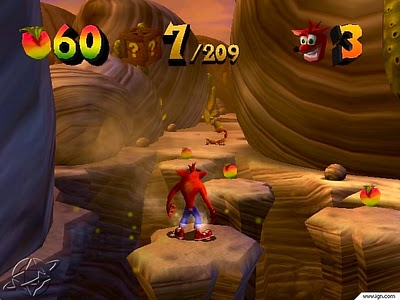
\includegraphics[scale=0.705]{Imagens/crash1.png}
 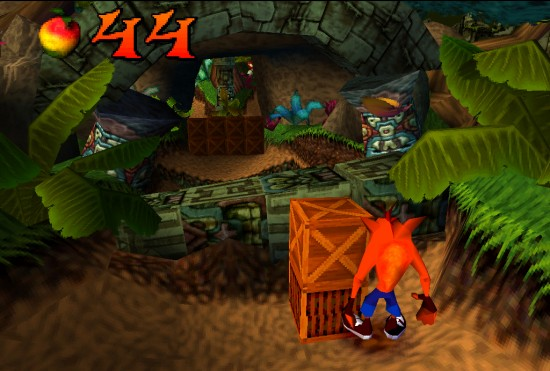
\includegraphics[scale=0.57]{Imagens/crash2.png}
 \caption{Captura de tela do jogo Crash Bandicoot 
(Fonte: \cite{bib:crash01,bib:crash02})}
 \label{img:crash}
\end{figure}

\item {\bf Super Mario Galaxy\cite{bib:mario_game}}
O jogo Super Mario Galaxy 
um jogo de aventura 3D é produzido pela Nintendo EAD Tóquio. A ação se passa 
em terceira pessoa e o jogador deve controlar o personagem em uma aventura 
galáctica para salvar a princesa Peach.
Este jogo, eleito o melhor jogo da história da Nintendo, conta com diversificados 
efeitos gravitacionais que proporcionam uma jogabilidade diferenciada, assim como 
é demonstrado na figura \ref{img:mario}. É importante ressaltar que como o jogo acontece no 
espaço, cada planeta tem suas características próprias, como por exemplo, 
gravidades diferentes. 
Esta jogabilidade permite jogos de câmeras não convencionais, movimentando a
 mesma de acordo com a posição do jogador e também do ``corpo celeste'' em que
 este se encontra.
Nas imagens abaixo é possível observar capturas de tela do Super Mario Galaxy.

\begin{figure}[!ht]
 \centering
 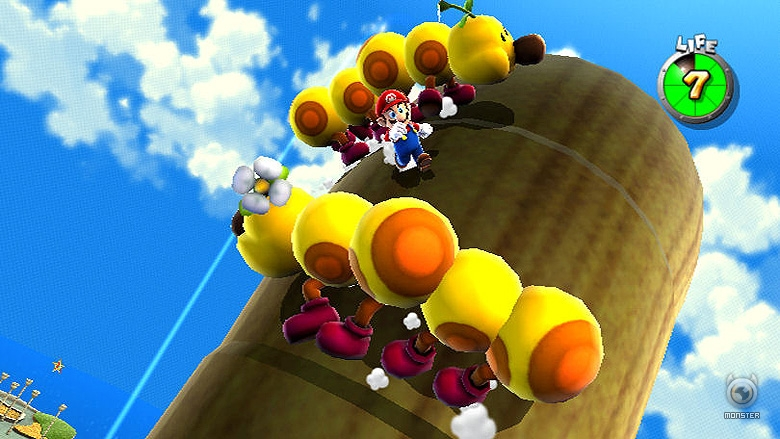
\includegraphics[scale=0.4]{Imagens/mario1.png}
 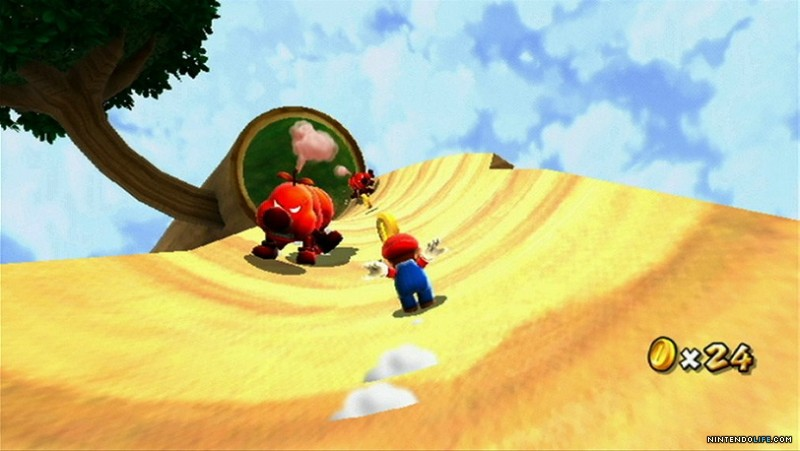
\includegraphics[scale=0.4]{Imagens/mario2.png}
 \caption{Captura de tela do jogo Super Mário Galaxy.
(Fonte: \cite{bib:mario01,bib:mario02})}
 \label{img:mario}
\end{figure}

\item {\bf Zelda\cite{bib:zelda_game}}
Dos jogos utilizados como referência para o desenvolvimento de
 ``As Crônicas de Medrash'',
é o que conta com maior liberdade de movimentação, embora ainda conte com 
caminhos específicos e ações determinadas a serem seguidas.
Neste jogo ocorre uma mistura a partir de uma trama complexa utilizando 
elementos de jogos de aventura com elementos de jogos de estratégia, os RPG. 
Esta mistura de gêneros faz com que Zelda se destaque com sua jogabilidade e
 possibilidades de exploração de habilidades do jogador. 
A série Zelda apresentou algumas características inovadoras. Em um dos jogos
 da série Zelda, o Ocarina of Time, o jogador utiliza-se de mira fixa, uma diferença 
com relação ao Mário 64, por exemplo.
Na Figura \ref{img:zelda} constam exemplos da ação no jogo Zelda.

\begin{figure}[!ht]
 \centering
 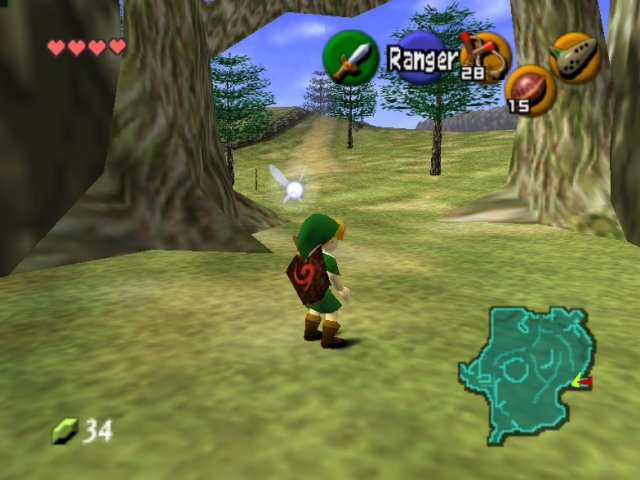
\includegraphics[scale=0.35]{Imagens/zelda1.png}
 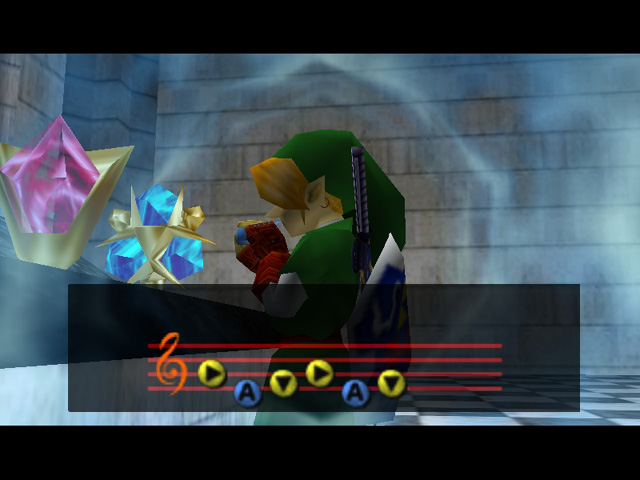
\includegraphics[scale=0.35]{Imagens/zelda2.png}
 \caption{Captura de tela do jogo Legend of Zelda.
(Fonte: \cite{bib:zelda01})}
 \label{img:zelda}
\end{figure}

\item {\bf Pitfall 3D\cite{bib:pitfall_game}}
Pitfall 3D
 é um jogo onde o desafio é manipular o personagem através de uma floresta 
que se dispõe como um tipo de labirinto. Para vencer o jogador deve recolher 
tesouros em um determinado espaço de tempo vencendo desafios (poço de piche, 
areia movediça, buracos, troncos de árvore rolando, cascavel, escorpião, fogo, 
morcego e crocodilo).
O jogo ``As Crônicas de Medrash'' se desenvolve de maneira parecida, exigindo 
além da orientação do personagem no mapa a coleta de itens como alimento e fogo,
 mantendo-se com vigor para continuar a jogar.

\begin{figure}[!ht]
 \centering
 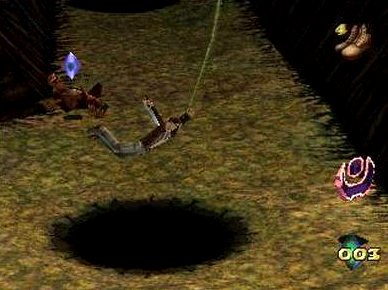
\includegraphics[scale=0.62]{Imagens/pit1.png}
 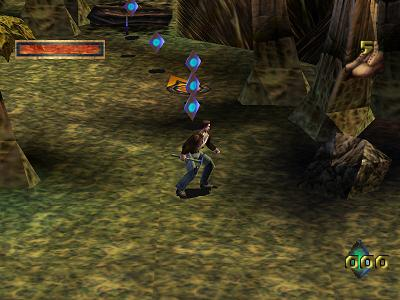
\includegraphics[scale=0.6]{Imagens/pit2.png}
 \caption{Captura de tela do jogo Pitfall 3D}
 \label{img:pitfall}
\end{figure}

\end{itemize}


% 1.2 Características Gerias (Escopo) / Som
% 1.3 Referências / Som
\section{Personagens}

\subsection{Introdução}
O jogo apresentará duas classes de dificuldades ao personagem principal 
(ou jogador): de percurso e de inimigos. As dificuldades de percurso serão 
aquelas apresentadas pelo ambiente e que exigirá a habilidade de locomoção 
do personagem, tal como salto ou desvio de obstáculos. As dificuldades 
de inimigos serão aquelas que exigirão a habilidade de ataque e defesa 
do personagem quando em confronto com um inimigo.

Nas seções a seguir são apresentadas as formas de controle dos estados 
do personagem principal, os inimigos e suas respectivas características 
e, por fim, o cenário e seus desafios.

\subsection{Estados do personagem principal}
Na primeira fase do jogo, haverá duas barras para que o jogador possa 
controlar os estados do personagem principal, ou seja, a condição física 
dele: a barra de vida e a barra de energia.
 
\subsubsection{Barra de Vida}
A barra de vida exibe o nível de vitalidade do personagem principal. 
A \ref{img:energia} apresenta um esboço desta barra, que começa completa, com
100 pontos percentuais. São dois os fatores que influenciarão no 
decaimento do nível: ataques sofridos e barra de energia vazia. Os ataques 
sofridos condizem com os ataques dos animais e inimigos que o personagem encontrará
nos cenários. O valor que será decrementado da barra de 
vida dependerá da força de ataque recebido, que varia de acordo com o oponente. 
Sobre a barra de energia vazia e a forma de recuperação da força vital do personagem, 
estas são tratadas na subseção a seguir.

\begin{figure}[H]
 \centering
 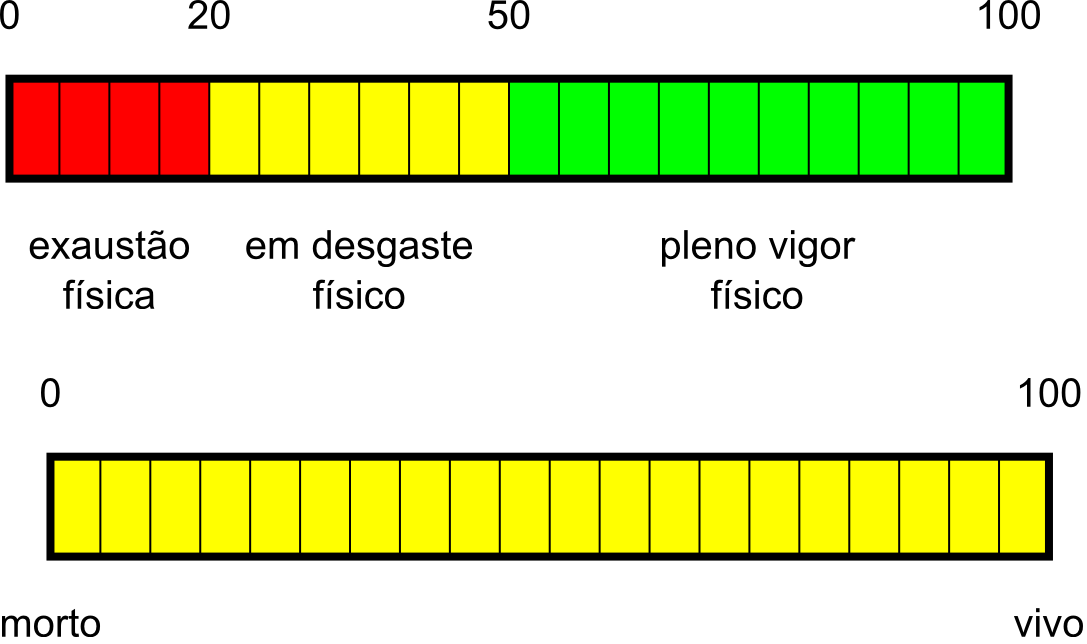
\includegraphics[scale=0.3]{BarraDeEnergia.png}
 \caption{Esboço das barras de vida (acima) e energia (abaixo).}
 \label{img:energia}
\end{figure}

\subsubsection{Barra de Energia}
A barra de energia exibe o nível de resistência física do personagem principal, 
ou seja, a capacidade dele para desenvolver um esforço físico. A \ref{img:energia} 
apresenta um esboço desta barra, que inicia cheia. No intervalo de 50 a 100, destacado em 
verde, o personagem estará em pleno vigor físico. Ele conseguirá correr e pular 
alto ou longas distâncias. No intervalo de 20 a 50, destacado em amarelo, o 
personagem começará a sofrer um desgaste físico. Ele passará a correr cada vez 
mais lento e a saltar alturas e distâncias cada vez menores até chegar à exaustão 
física - a função para controle da capacidade de esforço físico do personagem é 
apresentada na \ref{img:velocidade}. No intervalo de 0 a 20, o personagem já não conseguirá 
mais correr e nem pular, apenas andar.

\begin{figure}[H]
 \centering
 \includegraphics[scale=2.5]{VelocidadeDeDeslocamentoEPulo.png}
 \caption{Relação entre a capacidade de esforço físico e a energia
do personagem.}
 \label{img:velocidade}
\end{figure}

Os fatores que influenciarão no decaimento do nível de resistência física 
do personagem são: deslocamento, pulo e golpe. No deslocamento, o nível de 
energia deverá reduzir linearmente em função da distância percorrida pelo 
personagem. A cada pulo ou golpe realizado pelo personagem será decrementado 
ao nível de energia 1 e 1/2 ponto percentual, respectivamente. Se a barra de 
energia estiver vazia, estes fatores deverão interferir, na mesma proporção, 
no nível de vitalidade do personagem. Para elevar ambos os níveis de 
resistência física e de vitalidade, o personagem deverá matar e, em 
seguida, se alimentar dos animais que ele encontrará pelo caminho. Cada 
animal tem o seu valor energético específico.

\subsection{Personagens}
Na primeira fase, os inimigos do personagem principal serão os animais da floresta. 
Haverá cinco espécies de animais: cobra, urso, abelha, jacaré e tigre. Cada espécie 
terá suas características específicas. Estas são apresentadas na \ref{img:tabela}, em que K 
é um valor constante e p.p. é a abreviação de pontos percentuais.

\begin{figure}[H]
 \centering
 \includegraphics[scale=1]{tabela.png}
 \caption{Características dos animais selvagens}
 \label{img:tabela}
\end{figure}

\subsection{Personagem principal}
\subsubsection{Descrição física e psicológica}
Medrash é o personagem principal, que será controlado pelo jogador. Ele
 possui cerca de 20 anos de idade, 1,65 m de altura e 70 Kg. Com um corpo
 magro, mas com músculos definidos, é muito forte, sendo tipicamente um
 caçador.

Ele é um caçador da tribo Ari e marido de Sora. Medrash tem sua esposa e
 amigos sequestrados no inicio do jogo e seu objetivo principal é 
resgatalos.

Medrash enfrenta diferentes inimigos ao longo do jogo. É corajoso,
 determinado e não desiste de resgatar seus companheiros mesmo diante de
 todos os perigos enfrentados ao longo do caminho. É um homem bom e astuto,
 oferecendo ajuda a uma tribo aliada e juntando forças com os mesmos a fim
 de enfrentar a poderosa tribo Luskan.

\subsubsection{Concepção artística}
O Modelo base de Medrash é mostrado na figura \ref{img:medrash}

\begin{figure}[H]
 \centering
 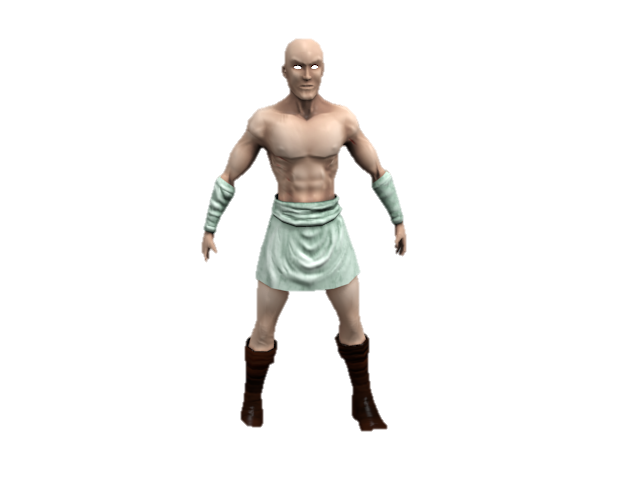
\includegraphics[scale=1]{Imagens/medrash01.png}
 \caption{Medrash. (Fonte: \cite{bib:medrash01})}
\label{img:medrash}
\end{figure}

\subsubsection{Armas do personagem principal}
\begin{itemize}
\item {\bf Porrete}
O porrete é a arma inicial de Medrash. Simples, rápida e fácil de usar,
 esta arma pode ser utilizada para atacar a maior parte dos inimigos da
 primeira fase.

A Figura \ref{img:porrete} mostra uma concepção artística desta arma.

\begin{figure}[H]
 \centering
 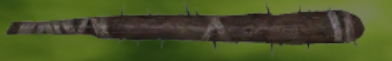
\includegraphics[scale=1]{Imagens/porrete01.png}
 \caption{Exemplo de porrete.  (Fonte: \cite{bib:jogoinfinity})}
\label{img:porrete}
\end{figure}

\item {\bf Lança}
A lança é a segunda arma de Medrash, encontrada ainda na primeira fase,
 podendo ser adquirida de um guerreiro morto. Ela apresenta um grande poder
 de perfuração, sendo assim, mais eficiente que o porrete para caçar
 tigres.

A concepção artistica da lança está na figura \ref{img:lanca}.

\begin{figure}[H]
 \centering
 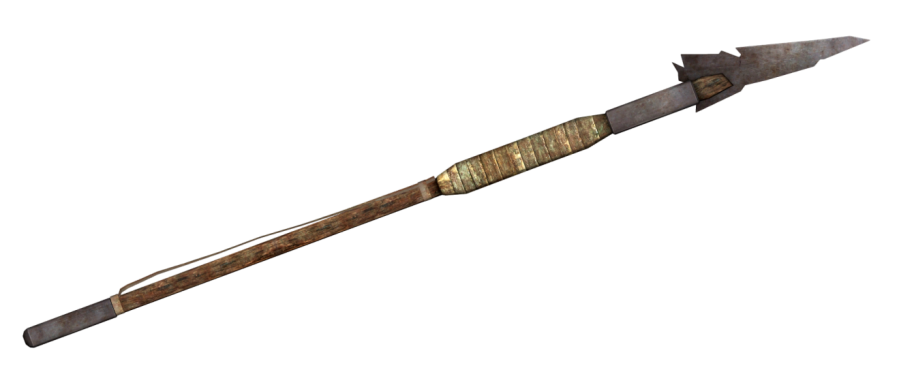
\includegraphics[scale=0.6]{Imagens/lanca01.png}
 \caption{Exemplo de lança. (Fonte: \cite{bib:lanca01})}
\label{img:lanca}
\end{figure}


\item {\bf Machado}
Esta arma é adquirida na segunda parte da fase 2. O machado é umas das mais
 poderosas armas de 
medrash e é com ela que nosso herói deverá enfrentar seus principais
 inimigos desta fase: os guerreiros da furiosa tribo Lauskan

O conceito artístico do machado pode ser encontrado na figura 
\ref{img:machado}.

\begin{figure}[H]
 \centering
 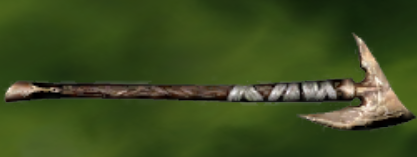
\includegraphics[scale=1]{Imagens/machado01.png}
 \caption{Exemplo de machado. (Fonte: \cite{bib:jogoinfinity})}
\label{img:machado}
\end{figure}

\end{itemize}

\subsection{Personagens secundários}
\subsubsection{Sora}
Sora é mulher de Medrash, que vive pacificamente na tribo Ari. Sequestrada
 por Balazar para ser escravizada, precisa da ajuda de Medrash para poder
 ser livre novamente.
\begin{itemize}
\item {\bf Descrição física}
Com aproximadamente 18 anos, com 1.55 m de altura e 50 Kg, 
\item {\bf Concepção artística}
O modelo de Sora é demonstrado na figura \ref{img:sora}.

\begin{figure}[H]
 \centering
 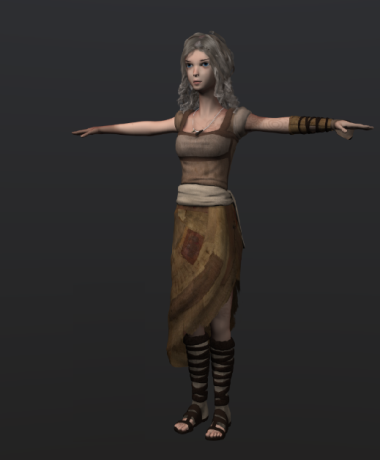
\includegraphics[scale=0.8]{Imagens/sora01.png}
 \caption{Sora. (Fonte: \cite{bib:sora01})}
\label{img:sora}
\end{figure}


As animações para este personagem são:
\begin{itemize}
\item Ficar parada (gritando, movimentando-se);
\item Corre.
\end{itemize}
\end{itemize}

\subsubsection{Gardain}
Um dos principais guerreiros da tribo Ari, a tribo de Medrash, e o único
 sobrevivente do ataque da tribo Luskan. Ao retornar de sua caçada, Medrash
 vê sua tribo totalmente devastada, restando apenas Gardain como
 sobrevivente. Mesmo estando muito machucado, Gardain conta a Medrash que
 os Luskans fizeram todos da tribo prisioneiros, inclusive sua amada Sora. 
\begin{itemize}
\item {\bf Descrição Física}
Gardain é um guerreiro forte, porém, devido a batalha com a tribo Luskan
 encontra-se esgotado e com diversos ferimentos pelo corpo.
\item {\bf Concepção Artística}
O modelo que servirá como base para a criação de Gardain é apresentado na
 Figura \ref{img:gardain}. Alterações de vestimenta e maiores detalhes
 serão acrescentados para a concepção do personagem.

\begin{figure}[H]
 \centering
 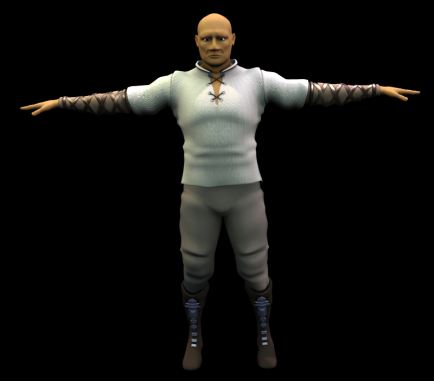
\includegraphics[scale=1]{Imagens/gardain01.png}
 \caption{Modelo para a criação de Gardain. (Fonte: \cite{bib:gardain01})}
\label{img:gardain}
\end{figure}


\end{itemize}
\subsubsection{Rangrim}
Rangrim é o líder da tribo dos Mara-kai. Ao chegar na tribo, Medrash
 encontra-o ferido após o ataque da tribo Luskan. Rangrim informa Medrash de
 que os Luskan pretendem atacar a tribo aliada Akanul, a maior e mais
 importante da região. Experiente e sábio, Rangrim conhece bem os caminhos
 e perigos da região, e indica a Medrash um atalho através das montanhas
 Kabalus, o que permitirá que Medrash chegue a tribo Akanul muito antes dos
 Luskans.
\begin{itemize}
\item {\bf Descrição Física}
Ancião, Rangrim é magro e de baixa estatura. Cabelos e barba branca,
 Rangrim anda de maneira curvada devido a idade avançada.
\item {\bf Concepção Artística}
O ancião apresentado na Figura \ref{img:rangrim} será utilizado para a criação
 do personagem Rangrim. Alterações de vestimenta serão realizadas para que
 se adeque ao período do jogo.

\end{itemize}
\begin{figure}[H]
 \centering
 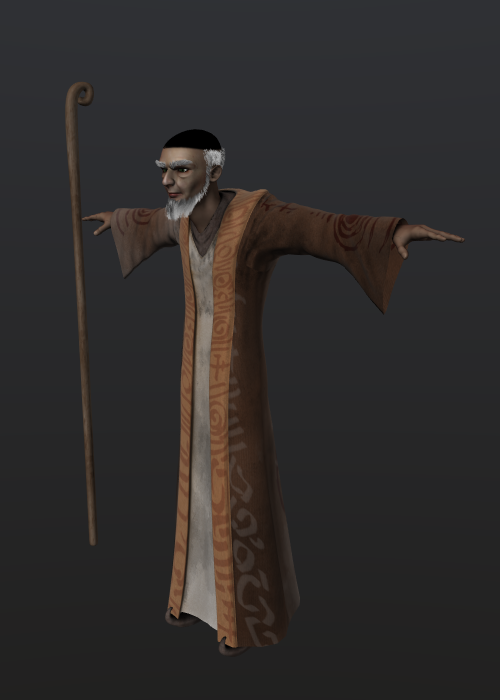
\includegraphics[scale=0.5]{Imagens/rangrim01.png}
 \caption{Modelo de ancião para a criação do personagem Rangrim. (Fonte: \cite{bib:rangrim01})}
\label{img:rangrim}
\end{figure}

\subsection{Inimigos}
\subsubsection{Cobra}
Não é um inimigo direto de Medrash, só ataca quando se sente ameaçada. A
 cobra é a segunda menor criatura do jogo atrás apenas da abelha. Ela
 patrulha uma determinada área rastejando e, caso o personagem principal se
 aproxime, esta fica enrolada em posição de ataque efetuando bote em forma
 de mordida caso a distância diminua. Se o personagem principal se
 distanciar a cobra volta a patrulhar a área. A cobra está presente apenas
 na primeira fase do jogo.
\begin{itemize}
\item {\bf Descrição Física}
Como mencionado, a cobra é um dos menores inimigos de Medrash. Medindo
 cerca de 80 cm, tem aparência realista e possui presas afiadas para o seu
 único ataque, a mordida. A tabela \ref{table:cobra} apresenta as principais
 características da cobra, onde K é um valor constante e p.p. é a
 abreviação para pontos percentuais.
\begin{table}[H]
\begin{center}
\begin{tabular}{|c|c|}
\hline 
\textbf{Característica} & \textbf{Valor} \\ 
\hline 
Raio de detecção do personagem principal & K \\ 
\hline 
Raio de perda de detecção do personagem principal & 1,5K \\ 
\hline 
Valor energético para o personagem principal & +30 p.p. \\ 
\hline 
Número de golpes para morrer & 3 \\ 
\hline 
Forma de ataque & Mordida \\ 
\hline 
Tipo de dano & Contusão \\ 
\hline 
Valor do dano & -5 p.p. \\ 
\hline 
\end{tabular} 
\end{center}
\caption{Características da Cobra}
\label{table:cobra}
\end{table}
\item {\bf Concepção Artística}
O modelo da cobra é mostrado abaixo:


\begin{figure}[H]
 \centering
 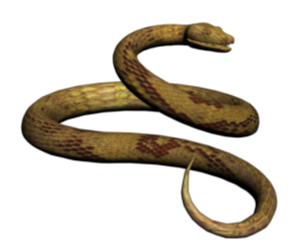
\includegraphics[scale=0.7]{Imagens/cobra01.png}
 \caption{Modelo da Cobra. (Fonte: \cite{bib:cobra01})}
\label{img:cobra}
\end{figure}


As animações para este personagem são:
\begin{itemize}
\item Rastejar;
\item Enrolar para o ataque;
\item Bote/Ataque;
\end{itemize}
\end{itemize}

\subsubsection{Urso}
O urso é o maior inimigo de Medrash e está presente somente na primeira
 fase do jogo. Se Medrash se aproximar muito dele, o urso se defenderá,
 perseguindo Medrash. Ao alcança-lo, o urso o ataca. O distanciamento de
 Medrash faz o urso esquecê-lo, voltando a patrulhar a região do mapa.
\begin{itemize}
\item {\bf Descrição física}
O urso pesa aproximadamente 400 Kg, tendo até 4 m de altura quando em
 posição bípede. Ele é muito robusto e apresenta pelagem marrom.


\begin{table}[H]
\begin{center}
\begin{tabular}{|c|c|}
\hline 
\textbf{Característica} & \textbf{Valor} \\ 
\hline 
Raio de detecção do personagem principal & 2K \\ 
\hline 
Raio de perda de detecção do personagem principal & 6K \\ 
\hline 
Valor energético para o personagem principal & +90 p.p. \\ 
\hline 
Número de golpes para morrer & 9 \\ 
\hline 
Forma de ataque & Mordida \\ 
\hline 
Tipo de dano & Contusão \\ 
\hline 
Valor do dano & -15 p.p. \\ 
\hline 
\end{tabular} 
\caption{Características do Urso}
\end{center}
\end{table}


\item {\bf Concepção Artística}
O modelo definido para o urso é mostrado na Figura \ref{img:urso}.

\begin{figure}[H]
 \centering
 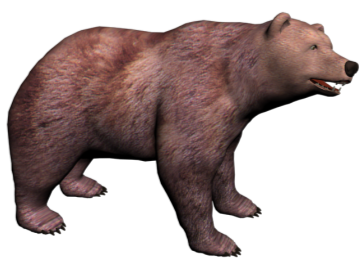
\includegraphics[scale=0.8]{Imagens/urso01.png}
 \caption{Modelo do urso. (Fonte: \cite{bib:urso01})}
\label{img:urso}
\end{figure}

As animações que o urso deverá ter são:
\begin{itemize}
\item Andar;
\item Correr;
\item Ficar sobre as patas traseiras;
\item Abraçar e morder Medrash.
\end{itemize}
\end{itemize}

\subsubsection{Jacaré}
O jacaré é um inimigo natural também encontrado na primeira fase do jogo.
 Vive dentro e ao redor de um rio, o qual Medrash é obrigado a atravessar para ir de
 um lado do cenário à outro. O jacaré basicamente fica parado à margem do rio, e/ou
 nadando nele. Da mesma forma que a cobra, o jacaré só ataca se Medrash
 chegar muito próximo dele, nesse caso ele começa a persegui-lo tanto
 dentro como fora d'água. Se Medrash estiver muito perto do jacaré, este
 irá atacá-lo, ou seja, irá abocanhar Medrash. Caso Medrash se distancie o
 jacaré volta à sua posição inicial.
\begin{itemize}
\item {\bf Descrição Física}
O jacaré também possui aparência realista, com cerca de 2m de comprimento e
 pesando 80 Kg. Possui dentes afiados e maior agilidade dentro da água.
 Fora dela se torna muito mais lento, porém possui o mesmo poder de ataque.
 A tabela \ref{table:jacare} descreve as principais características do jacaré.

\begin{table}[H]
\begin{center}
\begin{tabular}{|c|c|}
\hline 
\textbf{Característica} & \textbf{Valor} \\ 
\hline 
Raio de detecção do personagem principal & 0,5K \\ 
\hline 
Raio de perda de detecção do personagem principal & 6K \\ 
\hline 
Valor energético para o personagem principal & +60 p.p. \\ 
\hline 
Número de golpes para morrer & 6 \\ 
\hline 
Forma de ataque & Mordida \\ 
\hline 
Tipo de dano & Cortante/Contusão \\ 
\hline 
Valor do dano & -10 p.p. \\ 
\hline 
\end{tabular} 
\caption{Características do jacaré}
\label{table:jacare}
\end{center}
\end{table}

\item {\bf Concepção Artística}
Ainda não foi definido um modelo específico que representará o jacaré,
 porém, o modelo da Figura \ref{img:jacare} servirá como base para concepção do
 personagem.
\newpage
\begin{figure}[H]
 \centering
 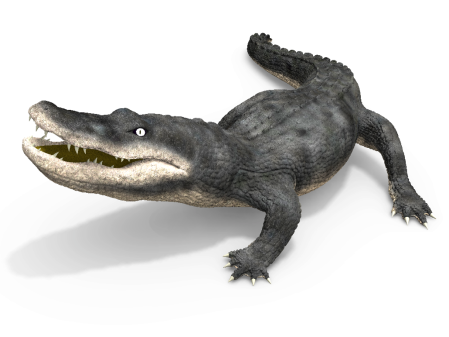
\includegraphics[scale=1]{Imagens/jacare01.png}
 \caption{Modelo do jacaré. (Fonte: \cite{bib:jacare01})}
\label{img:jacare}
\end{figure}

Animações que o jacaré deverá ter:
\begin{itemize}
\item Andar;
\item Nadar;
\item Abocanhar/Morder;
\end{itemize}
\end{itemize}
\subsubsection{Lobo}
O Lobo está presente na segunda fase do jogo, enquanto Medrash está cortando caminho pelas montanhas para chegar à tribo Akanul. O Lobo foge de Medrash sempre que este está com a tocha acesa. Quando ela apaga, ele o persegue por todo o cenário até que Medrash acenda a tocha novamente
\begin{itemize}
\item {\bf Descrição Física}
O Lobo apresenta uma altura de aproximadamente 75 centímetros, se medido a partir do ombro, pesando cerca de 30 Kg.
\begin{table}[H]
\begin{center}
\begin{tabular}{|c|c|}
\hline 
\textbf{Característica} & \textbf{Valor} \\ 
\hline 
Raio de detecção do personagem principal & 0,5K \\ 
\hline 
Raio de perda de detecção do personagem principal & 6K \\ 
\hline 
Valor energético para o personagem principal & +30 p.p. \\ 
\hline 
Número de golpes para morrer & 3 \\ 
\hline 
Forma de ataque & Mordida \\ 
\hline 
Tipo de dano & Cortante \\ 
\hline 
Valor do dano & -10 p.p. \\ 
\hline 
\end{tabular} 
\end{center}
\caption{Características do lobo}
\label{table:lobo}
\end{table}
\end{itemize}
\begin{itemize}
\newpage
\item {\bf Concepçao artística}
O modelo definido para o lobo é mostrado na \ref{img:lobo}.

\begin{figure}[H]
 \centering
 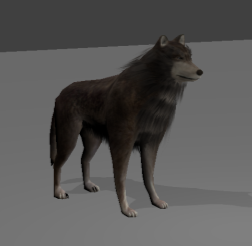
\includegraphics[scale=1]{Imagens/lobo01.png}
 \caption{Modelo do Lobo. (Fonte: \cite{bib:lobo01})}
\label{img:lobo}
\end{figure}


As animações que o lobo deverá ter:
\begin{itemize}
\item {Andar;}
\item {Correr;}
\item {Uivar;}
\item {Morder;}

\end{itemize}

\end{itemize}
\subsubsection{Enxame de abelhas}
Presente na primeira fase do jogo, na área do Urso, o enxame de abelhas vive tranquilamente, até Medrash se aproximar demais. As abelhas não são fortes, mas se Medrash não fugir rapidamente elas podem ser um problema.
\begin{itemize}
\item {\bf Descrição física}
A colméia das abelhas é de aproximadamente 40 cm, com uma aparência simples. As colméias apresentam cerca de 400 a 500 abelhas.

As abelhas são pequenas, com aproximadamente 1 cm. 
\begin{table}[H]
\begin{center}
\begin{tabular}{|c|c|}
\hline 
\textbf{Característica} & \textbf{Valor} \\ 
\hline 
Raio de detecção do personagem principal & 0,25K \\ 
\hline 
Raio de perda de detecção do personagem principal & 3K \\ 
\hline 
Valor energético para o personagem principal & Não convém\\ 
\hline 
Número de golpes para morrer & Não convém \\ 
\hline 
Forma de ataque & Picada \\ 
\hline 
Tipo de dano & Contusão \\ 
\hline 
Valor do dano & -1 p.p. \\ 
\hline 
\end{tabular} 
\end{center}
\caption{Características das abelhas}
\label{table:abelhas}
\end{table}
\end{itemize}
\begin{itemize}

\item {\bf Concepção artística}
O modelo de colméia será baseado na \ref{img:abelhas}.

 \begin{figure}[H]
 \centering
 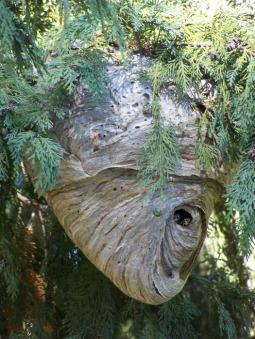
\includegraphics[scale=0.7]{Imagens/enxame01.png}
 \caption{Enxame de abelhas real. (Fonte: \cite{bib:enxame01})}
\label{img:abelhas}
\end{figure}
\end{itemize}
\newpage
\subsection{Tigre}
É o "chefe" da primeira fase, portanto o maior desafio para Medrash nesta etapa. Possui maior poder de ataque e é mais difícil de ser abatido.


O Tigre impede que Medrash avance para a próxima tribo (segunda fase), portanto, o jogador só poderá prosseguir caso derrote o Tigre. Medrash poderá usar a lança ou o porrete para derrotá-lo, sendo que com a lança os ataques são mais eficientes. O tigre possui um ataque mais poderoso, tirando mais pontos de vida de Medrash. O tigre desfere ataques em forma de mordida e saltando sobre Medrash.
\begin{itemize}
\item {\bf Descrição física}
O tigre possui tamanho e aparência de um tigre real, com cerca de 1,2 m de altura e 3 m de comprimento (incluindo a cauda), pesando 300 Kg.

A tabela \ref{table:tigre} traz as principais características do tigre.
\end{itemize}
\begin{table}[H]
\begin{center}
\begin{tabular}{|c|c|}
\hline 
\textbf{Característica} & \textbf{Valor} \\ 
\hline 
Raio de detecção do personagem principal & Não convém \\ 
\hline 
Raio de perda de detecção do personagem principal & Não convém \\ 
\hline 
Valor energético para o personagem principal & Não convém \\ 
\hline 
Número de golpes para morrer & 10 com a lança e 30 com o porrete \\ 
\hline 
Forma de ataque & Mordida/Patada\\ 
\hline 
Tipo de dano &  Contusão/Cortante \\ 
\hline 
Valor do dano & -15 p.p. \\ 
\hline 
\end{tabular} 
\end{center}
\caption{Características do Tigre}
\label{table:tigre}
\end{table}
\begin{itemize}
\item {\bf Concepção artística}

A figura \ref{img:tigre} demonstra o modelo do tigre.
\newpage
\begin{figure}[H]
 \centering
 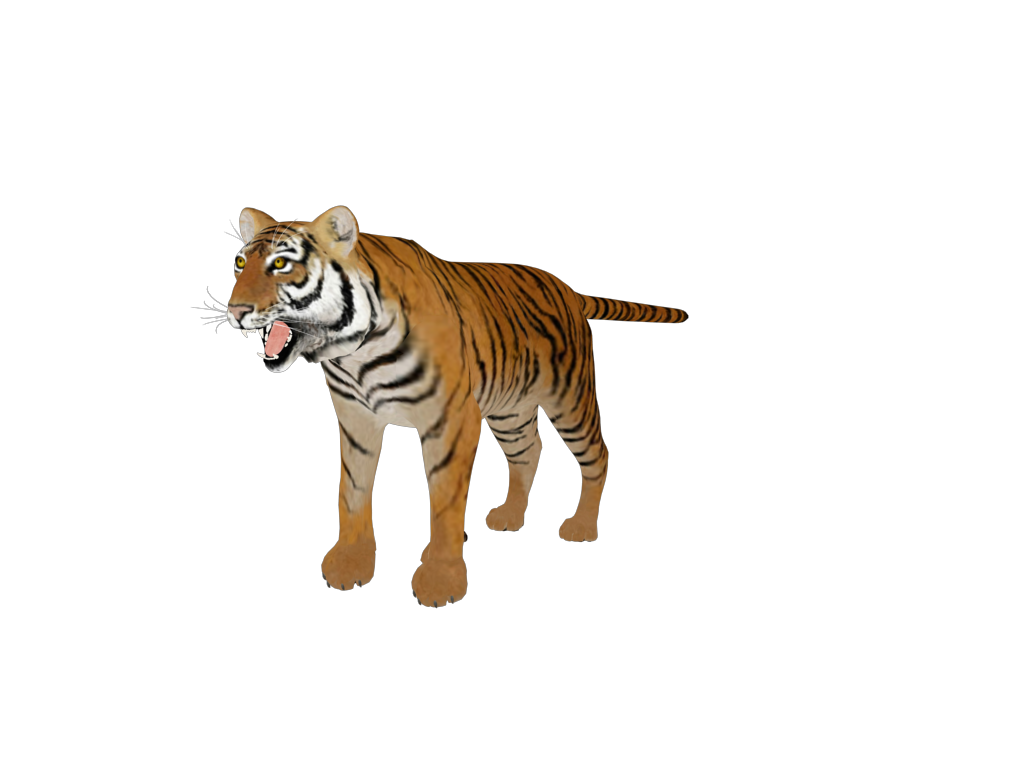
\includegraphics[scale=0.3]{Imagens/tigre01.png}
 \caption{Modelo do Tigre. (Fonte: \cite{bib:tigre01})}
\label{img:tigre}
\end{figure}

As animações do tigre são:
\begin{itemize}
\item {Andar;}
\item {Correr;}
\item {Posição para o ataque;}
\item {Ataque com salto;}
\item {Morder;}
\end{itemize}
\end{itemize}

\subsubsection{Balazar}
Balasar é o arqui-inimigo de Medrash. É o líder da tribo Luskan e tem como determinação destruir todas as outras tribos da região para se tornar líder absoluto. Balasar sequestra Sora e escraviza todos os outros.
\begin{itemize}
\item {\bf Descrição física}
Balazar é um personagem gordo, 1.65m de altura com 150 Kg.
\end{itemize}
\newpage
\begin{table}[H]
\begin{center}
\begin{tabular}{|c|c|}
\hline 
\textbf{Característica} & \textbf{Valor} \\ 
\hline 
Raio de detecção do personagem principal & Não convém \\ 
\hline 
Raio de perda de detecção do personagem principal & Não convém \\ 
\hline 
Valor energético para o personagem principal & Não convém \\ 
\hline 
Número de golpes para morrer & 15 com machado\\ 
\hline 
Forma de ataque & Ataque com porrete\\ 
\hline 
Tipo de dano &  Contusão/Cortante \\ 
\hline 
Valor do dano & -10 p.p. \\ 
\hline 
\end{tabular} 
\end{center}
\caption{Características de Balazar}
\label{table:balazar}
\end{table}
\begin{itemize}
\item{\bf Concepção artística} O modelo que representará Balazar é apresentado abaixo.
 \begin{figure}[H]
 \centering
 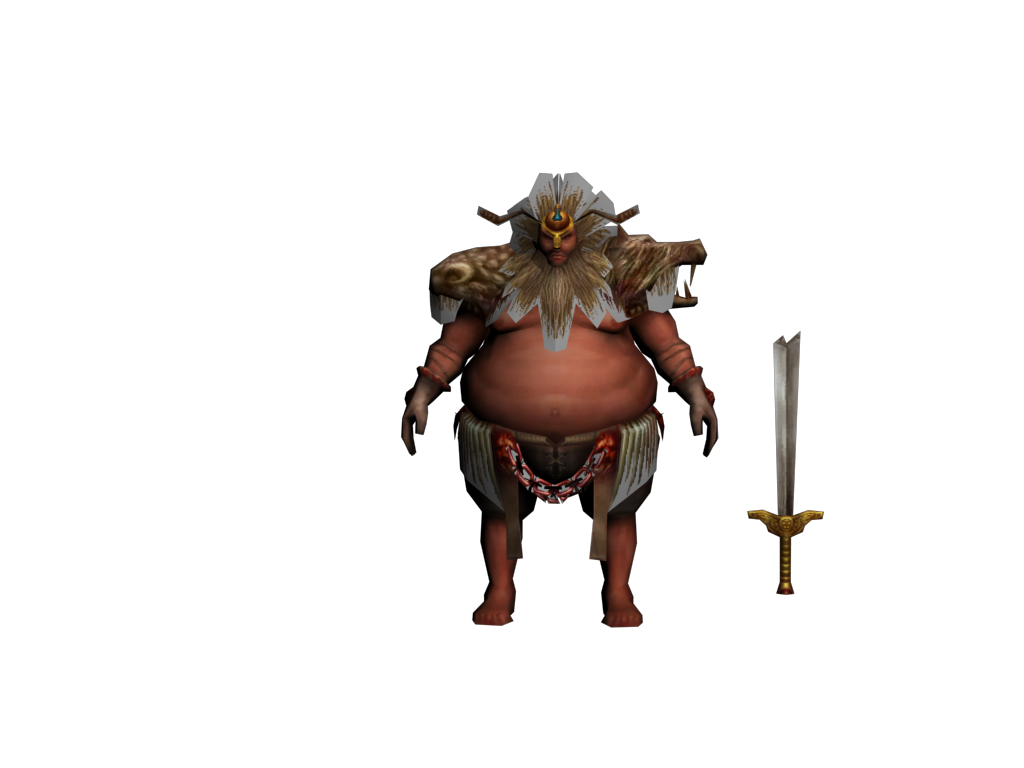
\includegraphics[scale=0.33]{Imagens/inimigo01.png}
 \caption{Modelo do Balazar. (Fonte: \cite{bib:balasar01})}
\label{img:balazar}
\end{figure}

Balazar deverá ter as seguintes animações: 
\begin{itemize}
\item {Atacar;}
\item {Atordoado;}
\item {Correr;}
\item {Cair;}
\end{itemize}
\end{itemize}
\subsubsection{Guerreiros inimigos da tribo Luskan}
Representam os humanos inimigos de Medrash. Dentre todos os inimigos da tribo Luskan, esses guerreiros são os mais fracos. Os guerreiros de Luskan aparecem no jogo a partir da parte dois da segunda fase, durante um ataque da tribo a tribo Mara-Kai. Nesse ataque participarão dois tipos de guerreiros da tribo Luskan, um que irá atear fogo na morada defendida por Medrash, e outro que entrará em combate direto com Medrash.

\begin{itemize}
\item{\bf Descrição física}
Esses guerreiros são os mais fracos da tribo Luskan. Com aproximadamente 1, 70m e pesando cerca de 70kg, possuem fisionomia muito parecida com a de Medrash. Seus ataques são baseados basicamente em luta corporal, mas podem também portar pequenas armas, porém, nada que se compare aos guerreiros mais fortes da tribo Luskan.
\end{itemize}

A tabela \ref{table:luskans} descreve as características básicas desses guerreiros.
\begin{table}[H]
\begin{center}
\begin{tabular}{|c|c|}
\hline 
\textbf{Característica} & \textbf{Valor} \\ 
\hline 
Número de golpes para morrer & 3\\ 
\hline 
Forma de ataque & Corporal\\ 
\hline 
Tipo de dano &  Contusão \\ 
\hline 
Valor do dano & -10 p.p. \\ 
\hline 
\end{tabular} 
\end{center}
\caption{Características dos guerreiros Luskans}
\label{table:luskans}
\end{table}
\begin{itemize}
\item{\bf Concepção artística}
O modelo que representará os guerreiros de Luskan é basicamente igual a de Medrash, com adaptações de vestimenta e armamento para se adaptar ao período do jogo.

Possivelmente será utilizado o mesmo modelo para essa classe de guerreiros, com algumas diferenciações apenas na forma física e/ou maneira de se vestir.

As figuras abaixo servirão de inspiração para a concepção dos modelos de guerreiros.
\newpage
 \begin{figure}[H]
 \centering
 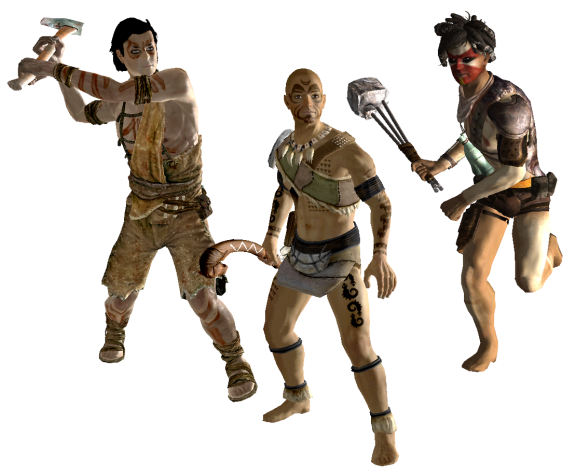
\includegraphics[scale=0.5]{Imagens/guerreiro01.png}
 \caption{Guerreiros tribais do jogo Fallout3. (Fonte:  \cite{bib:guerreiro01})}
\label{img:guerreiro01}
 \centering
 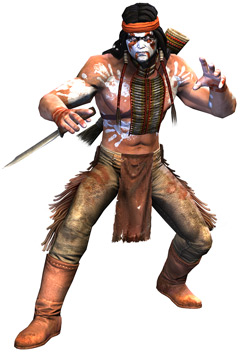
\includegraphics[scale=0.5]{Imagens/guerreiro02.png}
 \caption{Guerreiro Apache. (Fonte: \cite{bib:guerreiro02})}
\end{figure}
\end{itemize}

\subsubsection{Escravos}
Os escravos representam os habitantes das tribos Ari e Mara-kai que foram capturados pelos guerreiros da tribo Luskan. Os escravos estarão presentes na terceira fase do jogo, onde ficarão presos por estacas flamejantes. Serão divididos em três grupos. Nessa etapa Medrash deverá derrotar os inimigos da tribo Luskan para poder libertar os respectivos escravos. Tendo derrotado todos os guerreiros inimigos, Medrash poderá destruir as estacas que aprisionam os escravos, libertando-os.
\begin{itemize}
\item{\bf Descrição física}
Os escravos são humanos com a mesma aparência dos demais habitantes de sua tribo. Porém, devido ao aprisionamento, encontram-se visivelmente mais magros e debilitados.
\end{itemize}
\begin{itemize}
\item{\bf Concepção artística}
Como mencionado, os escravos serão modelos normais de humanos. Possivelmente sendo variações do modelo que representará os guerreiros inimigos, ou Medrash.


As imagens abaixo serão utilizadas como referência para a criação dos modelos.

\begin{figure}[H]
 \centering
 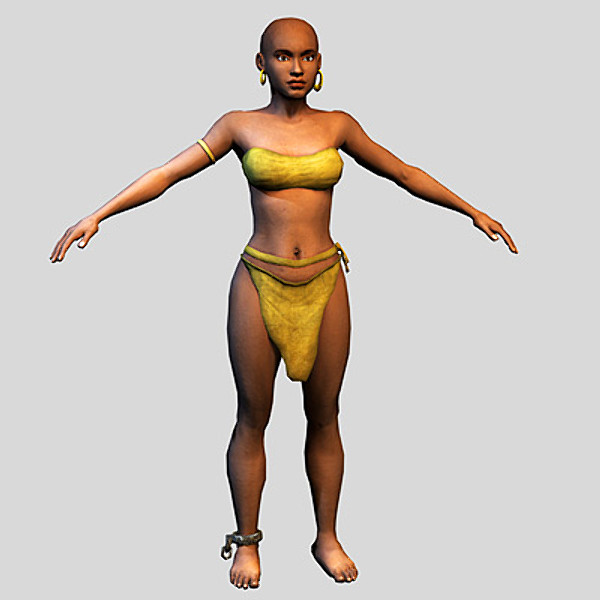
\includegraphics[scale=0.5]{Imagens/mulher01.png}
 \caption{Modelo de escrava. (Fonte: \cite{bib:escrava01})}
\label{img:mulher}
\end{figure}
\newpage
\begin{figure}[H]
 \centering
 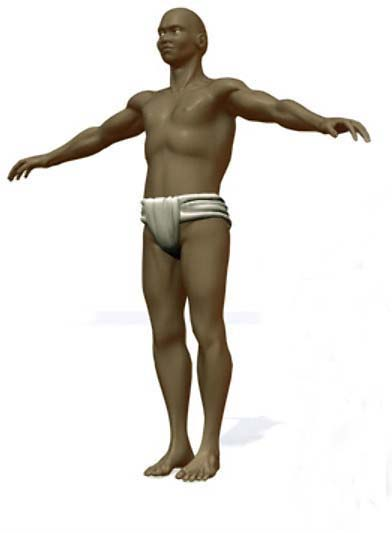
\includegraphics[scale=0.5]{Imagens/escravo01.png}
 \caption{Modelo de escravo. (Fonte: \cite{bib:escravo01})}
\label{img:escrava}
\end{figure}
\end{itemize}
\subsubsection{Porrete 2}
O porrete é a arma principal de Balazar. Esta arma apresenta um grande poder de destruição contra Medrash.

Abaixo é apresentada a arma de Balazar.

\begin{figure}[H]
 \centering
 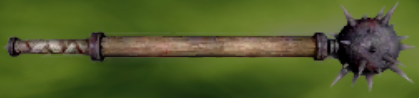
\includegraphics[scale=1]{Imagens/porrete02.png}
 \caption{Modelo de Porrete para Balazar (Fonte: \cite{bib:jogoinfinity})}
\label{img:porrete02}
\end{figure}
\section{Fases}

Nesta seção são apresentadas as descrições detalhadas das três fases do jogo.

\subsection{Fase 1}

Com nível de dificuldade baixo, a primeira fase representa a jornada de Medrash à tribo aliada Marakai pela floresta.

\subsubsection{Contextualização}

Após encontrar a sua tribo completamente destruída pelos guerreiros luskans, Medrash imediatamente começa uma jornada contra o tempo para tentar resgatar os membros de sua tribo -- que foram levados para serem escravizados -- antes deles chegarem na tribo Luskan. Medrash terá dois objetivos principais: chegar ao final da trilha deixada pelos guerreiros luskans e matar o tigre que o retardará de cumprir o objetivo anterior.

\subsubsection{Descrição do Espaço}

O espaço desta fase será uma floresta de coníferas. Esta será constituida de cinco regiões com suas próprias características : A, B, C, D e E, tal como esboçado no mapa da Figura \ref{fig:MapaDaFase1}. A região A, localizada na parte mais alta do mapa, é onde se encontra a tribo de Medrash e também é o ponto inicial do jogo. Para deslocar-se da região A à C, Medrash terá que passar obrigatoriamente pela região B, que é inclinada, cheia de rochas e infestada de cobras. A região C será plana e composta por muitas árvores. Esta área será dominada por ursos e em algumas ávores haverá cachos de abelhas. Na região D há um rio repleto de jacarés. Medrash poderá atravessá-lo andando (não correndo), já que as águas são baixas, ou pulando sobre as rochas no rio. Por fim, na reigão E, é onde encontra-se o último oponente de Medrash: o tigre. 

\begin{figure}[h]
\centering
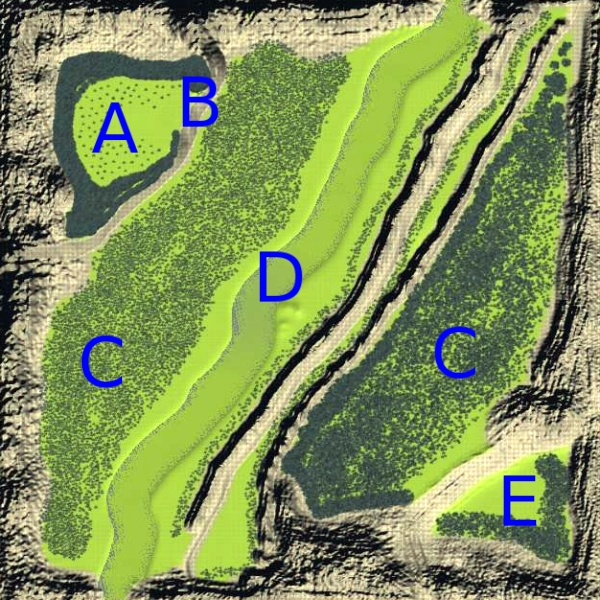
\includegraphics[width=10cm]{fases_mapa_1.jpg} 
\caption{Mapa da primeira fase}
\label{fig:MapaDaFase1}
\end{figure}

\subsubsection{Dificuldades ao Jogador}

As dificuldades de percurso serão as rochas soltas na descida da montanha onde esta localizada a tribo Ari, os cachos de abelhas espalhados pela floresta e as rochas sobre às águas do rio. As dificuldades de inimigos serão as cobras, ursos, jacarés e, no final, um tigre. O jogador também terá que administrar os medidores dos níveis de vitalidade e resistência física do Medrash, que estarão ativos nesta fase, exceto na etapa de enfrentamento do tigre, na qual apenas o primeiro estará ativo.

\subsubsection{Sequência dos Acontecimentos}

A seguir é apresentada a sequência dos acontecimentos da fase:

\begin{enumerate}
\item Uma animação ilustrará a chegada de Medrash à sua tribo Ari após uma longa caçada na mata. Ele encontrará seu amigo Gardain gravemente ferido em meio aos destroços da tribo. Gardain informará à Medrash o ocorrido e indicará o caminho que ele deverá seguir.
\item O jogador assume o controle de Medrash, que inicia com um porrete em mãos. Ele terá que seguir os rastros deixados pelos guerreiros invasores. Próximo à beira da montanha onde a tribo Ari está localizada, será possível avistar toda a floresta pelo qual Medrash deverá prosseguir.
\item Na descida da montanha haverão cobras e pedras soltas. Se Medrash cair, ele poderá morrer ou ficar gravemente ferido.
\item Após descer a montanha, Medrash estará em uma região plana dominada por ursos e cheia de cachos de abelhas.
\item Seguindo os rastros, Medrash chegará a um rio infestado de jacarés. Ele deverá atravesá-lo, seja andando pelas águas baixas ou saltando sobre as rochas.
\item Após a travessia, haverá continuidade dos rastros. Novamente haverá um região plana dominada por ursos e cheia de cachos de abelhas.
\item Próximo ao final da trilha, Medrash encontrará o corpo de um guerreiro morto. Junto a ele haverá uma lança, que o jogador poderá trocar pelo porrete.
\item No final da trilha haverá um tigre que impedirá a continuidade de Medrash. Ele deverá lutar com o tigre e matá-lo para finalizar a primeira fase.
\end{enumerate}

\subsection{Fase 2}

Com nível de dificuldade médio, a segunda fase representa a jornada de Medrash à tribo aliada Akanul pela montanha Kabalu.

\subsubsection{Contextualização}

Visando se adiantar à chegada dos guerreiros luskans na tribo Akanul -- última tribo aliada dos aris --, Medrash inicia uma jornada pela perigosa montanha Kabalu. Os objetivos principais de Medrash serão: cruzar a perigosa montanha a salvo e ajudar os guerreiros akanuls na defesa da tribo contra o ataque dos guerreiros luskans.

\subsubsection{Descrição do Espaço}

O espaço desta fase será a perigosa montanha Kabalu, que além de ser uma região de baixa temperatura, também é infestada de lobos selvagens. A Figura \ref{fig:MapaDaFase2} ilustra um esboço do mapa do local. A região A, representa a montanha Kabalu, cuja travessia é difícil, pois há fendas abertas no chão. E a região B representa a localização da tribo Akanul.

\begin{figure}[h]
\centering
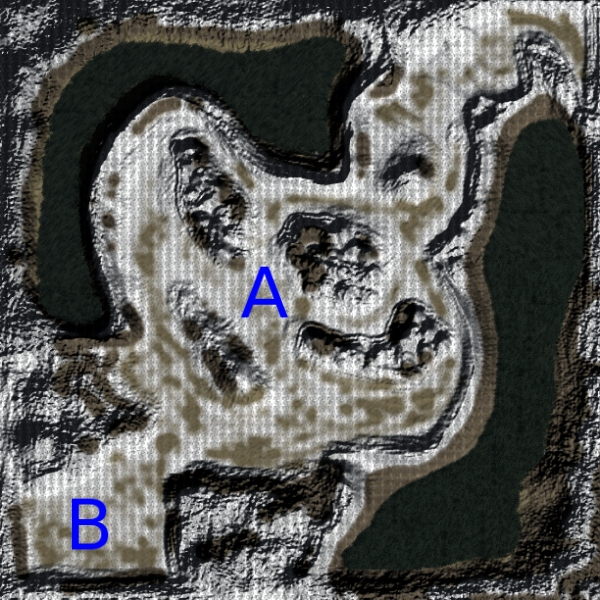
\includegraphics[width=10cm]{fases_mapa_2.jpg} 
\caption{Mapa da segunda fase}
\label{fig:MapaDaFase2}
\end{figure}

\subsubsection{Dificuldades ao Jogador}

As dificuldades de percurso serão as fendas abertas no chão e a baixa visibilidade do mesmo, já que o percurso será realizado de noite. As dificuldades de inimigos serão os lobos selvagens espalhados ao monte pela região e os guerreiros luskans que Medrash deverá infrentar no final da fase. O jogador também terá que administrar os medidores dos níveis de vitalidade e calor corpóreo do Medrash, que estarão ativos nesta fase, exceto na etapa de enfrentamento dos guerreiros luskans, na qual apenas o primeiro estará ativo.

\subsubsection{Sequência dos Acontecimentos}

A seguir é apresentada a sequência dos acontecimentos da fase:

\begin{enumerate}
\item Uma animação ilustrará Medrash avistando uma nuvem de fumaça ao longe. Ele correrá em direção a ela e verá os guerreiros luskans encerrando um forte ataque à tribo Marakai. Após a retirada dos lunkans, Medrash se aproximará da tribo e encontrará Rangrin gravemente ferido em meio aos destroços. Este o informará de que os luskans irão atacar a tribo Akanul e que Medrash deverá ir até ela pela montanha Kabalu para chegar antes deles.
\item O jogador assume o controle de Medrash. Medrash terá em mãos, além do porrete ou da lança, uma tocha acessa. Enquanto a tocha estiver acessa, os lobos não irão atacá-lo e a visibilidade do local próximo a ele será boa. Contudo, quando esta se apagar devido a rajadas de vento, os lobos perseguirão Medrash por toda região e a visibilidade das fendas no chão serão dificultosas. Medrash deverá acender a tocha em troncos de árvores atingidas por raios e ser rápido.
\item Ao atravessar a montanha, uma animação exibirá Medrash chegando à tribo Akanul e eles se preparando para o confronto.
\item O jogador novamente assume o controle de Medrash. Medrash terá em mãos um machado. Ele deverá proteger uma das moradias da tribo de guerreiros luskans que tentaram atear fogo nela.
\item Medrash deverá impedir que quatro desses guerreiros ateiem fogo na moradia para finalizar a fase.
\end{enumerate}

\subsection{Fase 3}

Com nível de dificuldade difícil, a terceira e última fase representa o contra-ataque dos guerreiros akanuls à tribo Luskan.

\subsubsection{Contextualização}

Como uma forma de retribuir à ajuda de Medrash, os guerreiros akanuls se unem ao herói e juntos partem em direção à tribo Luskan para contra-atacá-los. Já em território inimigo, enquanto os guerreiros akanuls e luskans confrontam-se, Medrash terá que cumprir dois objetivos: libertar os membros das tribos Ali e Marakai que foram capturados e aprisionados pelos guerreiros luskans; e enfrentar Balasar -- o temido líder dos luskans -- para resgatar a sua amada esposa Sora, que encontra-se aprisionada.

\subsubsection{Descrição do Espaço}

O espaço desta fase será o território da tribo Luskan. A Figura \ref{fig:MapaDaFase3} ilustra um esboço do mapa do local. A região A representa o local onde estarão as celas cujos membros das tribos Ari e Marakai estão aprisionados. A região B representa o local onde será o combate final entre Medrash e Balasar.

\begin{figure}[h]
\centering
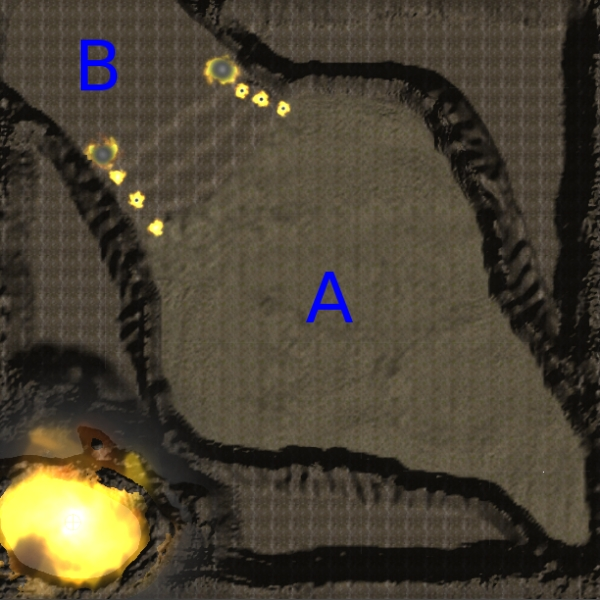
\includegraphics[width=10cm]{fases_mapa_3.jpg} 
\caption{Mapa da terceira e última fase}
\label{fig:MapaDaFase3}
\end{figure}

\subsubsection{Dificuldades ao Jogador}

As dificuldades de percurso serão as celas dos escravos e a lava do vulcão. As dificuldades de inimigos serão os guerreiros luskans, que impediram Medrash de libertar os membros das tribos, e Balasar. O jogador também terá que administrar os medidores do nível de vitalidade do Medrash e de tempo, que estarão ativos nesta fase, exceto na etapa de enfrentamento de Balasr, na qual apenas o primeiro estará ativo.

\subsubsection{Sequência dos Acontecimentos}

A seguir é apresentada a sequência dos acontecimentos da fase:

\begin{enumerate}
\item A fase começará com uma animação mostrando a chegada dos guerreiros akanuls e de Medrash no território dos luskans e o início do confronto.
\item O jogador assumirá o controle de Medrash, que encontra-se rodeado pelos combatentes, porém fora do alcance dos inimigos.
\item Assim que Medrash se aproximar demais de uma das três celas feitas de estacas de madeira, um guerreiro luskan ateará fogo na respectiva cela. O medidor de tempo será iniciado.
\item Outros guerreiros luskans irão atacar Medrash tentando impedí-lo de libertar os membros aprisionados.
\item Medrash precisará libertar os prisioneiros das três celas dentro do tempo para que possa prosseguir na fase. Se isto ocorrer, uma animação mostrará o vulcão entrando em erupsão e Balasar levando Sora para outro local. Medrash irá segui-lo. Ao chegar lá, Medrash verá sora aprisionada em uma cela.
\item O jogador assumirá novamente o controle de Medrash, que deverá enfrentar Balasar. Enquando ambos lutam, lava vulcânica irá escorrer para a direção de Sora. Medrash deve aproveitar enquando Balasar fica zonzo para bater nas estacas de madeira da cela.
\item Se Medrash conseguir destruir a cela há tempo que a lava não chegue até ela, então uma animação ilustrará Medrash aplicando um último golpe em Balasar, que cairá na lava. Por fim, ambos correm do local para ficarem a salvos do vulcão.
\end{enumerate}
\section{Fluxo do Jogo}
Este capítulo tem por objetivo descrever e mostrar a maneira como os diversos elementos que compõe o jogo interligam-se entre si.

\subsection{Progressão do Jogo}
Para a correta representação dos elementos que compõe o jogo um diagrama de máquinas de estados foi utilizado, o qual podem ser visualizado por meio da figura \ref{img:fluxo_jogo}.

\begin{figure}[!ht]
 \centering
 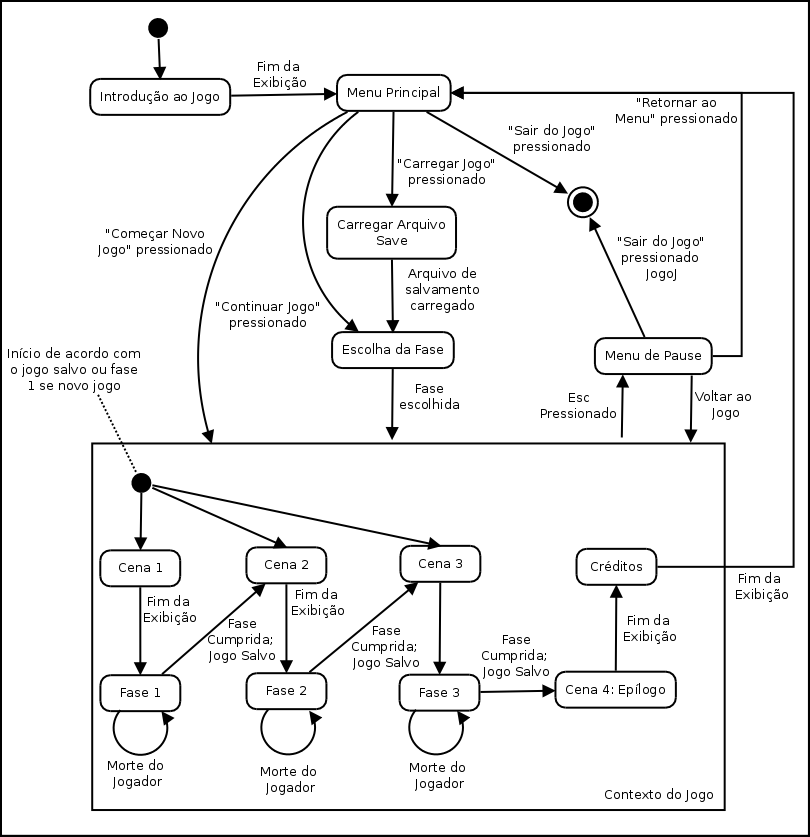
\includegraphics[scale=0.40]{fluxo_jogo.png}
 \caption{Diagrama do Fluxo do Jogo}
 \label{img:fluxo_jogo}
\end{figure}

Ao iniciar o aplicativo, o jogo tem início com a introdução e, logo após, passa o controle da interação ao menu principal. Neste menu, são previstas três opções: ``Começar um Novo Jogo'', ``Carregar Jogo'' e ``Sair''. ``Sair'' leva o personagem ao estado final do diagrama de máquina de estados, encerrando assim o aplicativo. ``Carregar Jogo'' permite ao jogador escolher um jogo salvo e passa, logo após, o controle à escolha das fases disponíveis no perfil carregado. ``Começar um Novo Jogo'' inicia uma nova campanha, onde o jogador é levado a assistir a cena 1, pela qual o enredo é apresentado. Após finalização desta, tem início à primeira fase. Com o decorrer do jogo,  diversas cenas e fases são alcançadas no caso de sucesso do usuário ao  cumprir os objetivos estabelecidos. Com a devida concretização da terceira fase, o epílogo e os créditos são apresentados, os quais devolvem, após finalizados, a interação ao controle do menu principal. Durante o jogo, com a eventual morte do personagem principal, o mesmo é levado ao último \textit{checkpoint} registrado. No caso da tecla Esc ser pressionada, a interação é pausada e, neste ponto, é possível retornar ao jogo, voltar ao menu principal ou sair para o ambiente de trabalho, finalizando assim o aplicativo.

No que diz respeito aos elementos contidos no fluxo do jogo representado pelo diagrama, os mesmos são elicitados e discutidos abaixo:
\begin{itemize}
\item \textit{Introdução ao Jogo:} a introdução é responsável por apresentar ao usuário informações referentes ao jogo em si, tais como a plataforma utilizada, os integrantes da equipe de trabalho, a disciplina e o professor;
\item \textit{Menu Principal:} o menu principal é o local onde são agrupados comandos que fornecem o ponto de partida ao jogo, com ações tais como "Começar um Novo Jogo" e "Carregar Jogo". É também o local onde o jogador é levado logo após a introdução inicial descrita acima;
\item \textit{Começar Novo Jogo:} opção do menu principal cujo acionamento leva o jogador à primeira etapa do contexto do jogo, o tutorial de aprendizado inicial. Ao escolher esta opção, o jogo se inicia;
\item \textit{Carregar Jogo:} opção do menu principal cujo acionamento possibilita ao jogador a escolher um jogo salvo. Esta opção permite ao jogador continuar uma ação interrompida em interações passadas;
\item \textit{Escolher Fase:} etapa de escolha de fase desejada, a qual torna-se disponível após a escolha do jogo salvo. Por meio dela é possível escolher dentre as fases já completadas que estiverem contidas dentro de um arquivo de jogo salvo;
\item \textit{Sair do Jogo:} opção presente tanto no menu principal, quanto no secundário, de \textit{pause}, a qual, em caso de acionamento, leva o jogador de volta ao ambiente de sua área de trabalho do sistema operacional, encerrando assim a execução do jogo;
\item \textit{Menu de Pause:} menu passível de ser acionado no evento de pressionar a tecla Esc do teclado. Sua função é manter o jogo pausado para posterior retorno ao contexto do jogo, se assim desejado pelo jogador. Outras opções são sair para o ambiente de trabalho e retornar ao menu principal;
\item \textit{Cena 1:} animação inicial utilizada para introduzir o usuário no contexto no jogo, contando o enredo e apresentando os personagens. Uma breve descrição para os eventos retratados pode ser dada por: Medrash volta para sua tribo, Ari, e encontra Gardain machucado, seu amigo, e o restante de seu grupo desaparecido. Gardain o informa que sua tribo foi atacado pela tribo Luskan e que seus amigos foram sequestrados, incluindo Sora, sua mulher;
\item \textit{Fase 1:} primeira fase jogável do jogo. Nela, o jogador deverá ir atrás de seus objetivos descritos na Cena 1, apresentada no item anterior, ou seja, deverá ir atrás dos inimigos que invadiram sua tribo e destruíram-na, levando seu povo e mulher como escravos;
\item \textit{Cena 2:} animação de transição da fase 1 para a fase 2. Retrata os acontecimentos que se sucedem ao jogador cumprindo a primeira fase com êxito. Uma descrição para ela pode ser dada por: Ao chegar na tribo Mara-kai, Medrash vê seus integrantes sendo atacados pelos Luskans.
\item \textit{Fase 2:} segunda fase jogável do jogo. Nela, o jogador deverá perseguir os objetivos descritos pelo contexto apresentado na Cena 2, apresentada no item anterior, ou seja, deverá ir percorrer as montanhas Kabalus em busca de um atalho para chegar antes que os inimigos à tribo aliada;
\item \textit{Cena 3:} animação de transição da fase 2 para a fase 3. Retrata o acontecimentos que se sucedem ao êxito do personagem ao cumprir a fase 2. Uma breve descrição para ela pode ser dada por: As tribos Akanul e Mara-kai se aliam para atacar Luskan;
\item \textit{Fase 3:} terceira fase jogável do jogo. Nela, o jogador terá que perseguir os objetivos e missões dadas na animação de introdução a ela (Cena 3, descrita no item anterior), ou seja, deverá deverá enfrentar seus inimigos no âmbito de salvar seus amigos e derrotar seu algoz, salvando assim, sua esposa;
\item \textit{Epílogo (Cena 4):} animação final retratando os acontecimentos com os personagens que se sucedem à fase 3, caso o jogador tenha sido bem sucedido ao cumprir suas missões no decorrer do jogo;
\item \textit{Créditos:} após concluir todas as fases com sucesso, o jogador será contemplado com os créditos de produção do jogo, contendo informações a respeito  da equipe de desenvolvimento, da disciplina e do professor orientador.
\end{itemize}

\subsection{Tempo de Jogo}
O jogo não possui um limite de tempo pré-definido, ou seja, ele não precisa ser cumprido dentro de um prazo estabelecido. Sendo verdade, o jogador fica livre para utilizar o tempo que desejar para cumprir todas as missões previstas. No entanto, com o jogador seguindo o percurso definido sem atrasos, estima-se uma duração total de aproximadamente 18 minutos, tendo as 2 primeiras fases uma duração aproximada de 6-8 minutos e a fase final 4-6 minutos.

\subsection{Condições de Vitória}
O jogador será considerado vencedor do jogo se permanecer vivo e vencer os obstáculos apresentados pelas 3 fases.

Na primeira fase o jogador deverá rastrear a trilha deixada por seus inimigos com o intuito de reaver seus amigos. Neste cenário ele não poderá morrer para qualquer um dos inimigos presentes e também terá que derrotar o chefe final, o tigre que bloqueia seu caminho, para ser bem sucedido.

Na segunda fase o jogador deverá pegar um atalho pelas montanhas afim de chegar a tempo para avisar os aliados do ataque que eles sofreriam. Neste cenário, ele não poderá morrer para nenhum inimigo que venha a lhe atacar no percurso e também terá que ser bem sucedido na defesa dos aliados, que irá ocorrer logo ao final da fase.

Na terceira e última fase o jogador deverá libertar os escravos e sua esposa das mãos dos inimigos. Neste cenário, ele não poderá morrer para nenhum obstáculo que tenha que enfrentar e terá que ser sucedido ao derrotar o chefe final, seu arqui-inimigo.

Ao completar as 3 fases com êxito, o jogador terá sido bem sucedido e será contemplado com o epílogo do jogo, o qual mostrará os acontecimentos que se sucederam à batalha final.

\subsection{Morte do Personagem Principal}
Caso o personagem principal morra em qualquer de uma das fases, o mesmo voltará ao último \textit{checkpoint} registrado durante a interação. As fases foram definidas para terem estes pontos antes do enfrentamento dos chefes de cada uma delas. 

\section{Mecânica do Jogo}

Nesta sessão serão descritas as regras de interação entre o jogador e o jogo.

\subsection {Mecânica Básica}

O jogador irá passar por mapas do jogo tendo a liberdade de se deslocar em
 qualquer direção dentro da área permitida.

\subsubsection {Controles}

O jogador poderá movimentar o personagem pelo cenário por meio das setas
 direcionais. Para as demais interações serão utilizadas as teclas
 ``A'', ``S'', ``D'' e a barra de espaço:
\begin{itemize}
\item {\bf ``A'' é o botão de ataque} O personagem utiliza a arma disponível
para atacar o inimigo mais próximo;
\item {\bf ``S'' é o botão de ação} O personagem realiza a interação com o
 cenário e outros personagens;
\item {\bf ``D'' é o botão de defesa} Quando não for possível sair da frente
 de um ataque, a tecla ``D'' pode ser usada para se defender;
\item {\bf A barra de espaço é o botão de pulo} O personagem pula.
\end{itemize}

\subsubsection {Deslocamento}
Na primeira fase o personagem principal se desloca inicialmente correndo. 
Conforme este perde energia, passa a correr mais devagar até que atinja um 
nível crítico onde passa apenas a andar. Nas demais, não haverá indicador 
de canseira.

\subsubsection {Inimigos e Desafios}
Nos mapas irão existir diversos inimigos que podem detectar o jogador caso 
este chegue muito próximo. Sendo verdade, eles iniciam uma perseguição. Assim 
que o jogador se afasta a uma determinada distância, os inimigos voltam ao 
seu estado inicial. 

Os inimigos quando próximos do jogador irão atacá-lo, possibilitando que o 
personagem também faça o mesmo. 
Adicionalmente, no final de cada mapa haverá um desafio extra, como um inimigo
 mais forte ou uma batalha.  

\subsubsection {Interação com o Cenário}

Além dos inimigos, o personagem principal poderá interagir com partes do
 cenário e NPCs para completar os desafios propostos.

\subsection {Combate}
\subsubsection{Inimigos}
Ao se aproximar dos inimigos, estes irão atacar o personagem principal. A
tecla ``A'' pode então ser pressionada para atacar o mais próximo.

Os ataques dos inimigos serão periódicos, podendo ser defendidos utilizando a
 tecla ``D'', que irá reduzir o dano causado. Também podem ser esquivados
 utilizando as setas direcionais para sair da região de efeito do ataque.

\subsection {Dificuldade}
O jogo apresentará duas classes de dificuldades ao personagem principal: de percurso e de
inimigos. As dificuldades de percurso serão aquelas apresentadas pelo ambiente e que exigirão a habilidade
de locomoção do personagem, tais como salto ou desvio de obstáculos. As dificuldades de inimigos serão
aquelas que exigirão a habilidade de ataque e defesa do personagem quando em confronto com um inimigo.

De uma fase para outra serão introduzidas novas mecânicas de jogo aumentando o
grau de dificuldade e criando um incentivo para que o jogador não perca o interesse pelo jogo.

\subsection {Vida, Energia e Temperatura}

Existem três barras principais durante o jogo: as barras de vida, energia e temperatura. 

A barra de vida indica a saúde do personagem. Esta barra diminui quando
o personagem sofre ataques dos inimigos e aumenta quando Medrash come os alimentos
encontrados.

A barra de energia representa um desafio extra durante a primeira fase. Esta
 barra diminui conforme o deslocamento do personagem e aumenta quando o 
mesmo cumpre algumas necessidades, tais como comer.

A barra de temperatura existe apenas na segunda fase e serve para mostrar que
o personagem está perdendo temperatura corporal. Esta barra aumenta quando o 
personagem aproxima-se do fogo.

\subsection {Salvar e Carregar o jogo}
Para salvar o progresso no jogo será utilizado um sistema de perfil. Inicialmente o jogador criará um perfil e este dará acesso à primeira fase. Após a conclusão das fases, as posteriores serão devidamente liberadas, com a opção de salvar o progresso obtido liberada. Somente é possível salvar um jogo no início de uma nova fase.

Será possível criar diversos perfis. Na tela inicial do jogo haverá uma opção de carregar o perfil e esta irá conter todos os existentes.
\section{Interface}

Nesta seção serão descritos os elementos da interação entre o jogador e o
jogo.

\subsection{HUD}

A tela do jogador terá as informações a seguir, seguindo o modelo da
Figura \ref{fig:hud}
\begin{figure}[!ht]
 \centering
 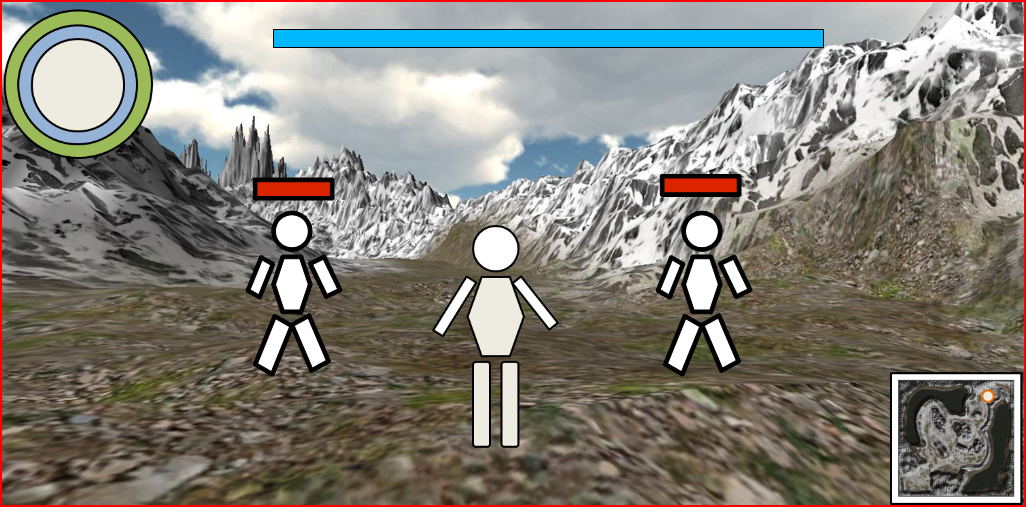
\includegraphics[scale=0.59]{hud.png}
 \caption{HUD}
 \label{fig:hud}
\end{figure}
\begin{enumerate}
 \item {\bf Marcador de vida:} Canto superior esquerdo da tela, no 
formato de uma faixa circular. Na figura está demonstrado pela faixa
verde;
 \item {\bf Marcador de energia/temperatura:} Quando houver este marcador,
ele estará no canto superior esquerdo da tela, também no formato
de uma faixa circular, dentro da faixa do marcador de vida. Na primeira
fase será o marcador de energia e, na segunda, o de temperatura. Não
existirá este marcador na terceira fase. Na figura está indicado pela 
faixa azul dentro da faixa verde;
 \item {\bf Minimapa:} Canto inferior direito, em forma de quadrado.
Será fixo e semi-transparente. Mostrará um esboço do mapa e um triângulo
indicando a posição e direção de Medrash. Existirá nas 3 fases;
 \item {\bf Barra de vida dos inimigos:} Ficará sobre a cabeça do inimigo,
indicando quantos pontos de vida ele ainda possui. Indicado na figura
como barras vermelhas;
 \item {\bf Barra de tempo:} Esta barra indicará indicará o tempo restante
 para completar a batalha final. Portanto, existe apenas na fase 3.
Seu tamanho irá diminuir progressivamente, indicando o tempo se esgotando. Na 
figura, a barra azul no topo da tela indica a Barra de Tempo.
\end{enumerate}

\subsection{Menus}

O jogo terá três menus. Um deles será o menu principal do jogo, o 
outro será o menu de pausa e o último será um menu entre fases.

\subsubsection{Menu Principal}

O menu principal terá as seguintes opções:
\begin{itemize}
 \item {\bf Começar novo jogo:} Apaga todas informações sobre o jogo atual
se houver e inicia um novo jogo;
 \item {\bf Continuar jogo:} Se houver um jogo em progresso, permite que
o usuário continue o mesmo. Caso contrário, esta opção estará desativada;
 \item {\bf Carregar jogo:} Permite que o usuário carregue algum jogo
gravado, se houver;
 \item {\bf Sair do jogo:} Sai do jogo, finalizando o software.
\end{itemize}

\subsubsection{Menu de Pausa}
O menu de pausa só pode ser acessado durante o jogo e contém as seguintes
opções:
\begin{itemize}
 \item {\bf Continuar o jogo:} Sai do menu de pausa;
 \item {\bf Voltar ao menu principal:} Sai do jogo e volta ao menu 
principal. Não salva o jogo;
 \item {\bf Sair do jogo:} Sai do jogo e finaliza o software.
\end{itemize}

\subsection{Menu entre fases}
Ao final das fases 1 e 2 será exibido um menu que irá mostrar a pontuação do
personagem, assim como as opções:
\begin{itemize}
 \item {\bf Salvar jogo:} Permite que o jogador salve o progresso;
 \item {\bf Próxima fase:} Continua para a próxima fase;
 \item {\bf Voltar ao menu principal:} Sai do jogo e volta ao menu principal;
 \item {\bf Sair do jogo:} Sai do jogo e finaliza o software.
\end{itemize}

\section{Músicas e Efeitos Sonoros/Trilha Sonora}

\subsection{Introdução ao tema}
A trilha sonora  é composta por todos os áudios presentes no aplicativo, 
tais como músicas (de menus ou de background), efeitos especiais, vozes 
e efeitos de personagens e narrações - quando houver necessidade.

A proposta da trilha sonora é criar ambiência, de modo a melhorar a imersão
 no jogo e garantir feedback mais eficiente e claro das ações tomadas pelo
 personagem (controlado pelo jogador), ações de inimigos, estímulos,
 obstáculos e NPCs
\footnote{Non-player character (Personagem não jogável) - compreende um 
personagem que não pode ser controlado pelo jogador, embora possa fazer
 parte da ação do jogo.}. 
A trilha sonora deve ainda valorizar o uso do software, de modo a permitir
 novas possibilidades de interação e comunicação com o usuário, indo além
 das informações visuais que não atenderiam ao uso do mesmo ou o tornaria
 seu uso menos interativo, mais lento e cansativo.

A narração é um componente da trilha sonora que deve ser produzido de forma
 cuidadosa, principalmente em jogos direcionados para público infantil ou
 em processo de alfabetização, pois guiará as ações do jogador e permitirá
 uma ação mais rápida e efetiva em caso de dúvidas ou orientações quanto
 ao jogo.

A produção da trilha sonora pode ocorrer de três maneiras:
\begin{itemize}
\item Captação do áudio da voz humana, de instrumentos musicais ou de
 objetos sonoros
\footnote{Compreendem objetos, que não são necessariamente instrumentos
 musicais, mas que emitem sons que podem ser aproveitados em criações
 artísticas e musicais. São elementos de criação estudados por diversos 
compositores, destacando-se Pierre Henri Marie Schaeffer.}, 
através de gravadores digitais ou computadores conectados com outros
 periféricos, como placa de som, microfones e mesas de som, utilizando-se
 de softwares específicos para isso: Sound Forge, Audacity, Sonar entre 
outros disponíveis no mercado. O resultado obtido normalmente é um 
arquivo de áudio.
\item Produção através de recursos MIDI
\footnote{Musical Instrument Digital Interface - compreende uma interface
 de comunicação entre dispositivos que se utilizem deste protocolo. 
Estes dispositivos podem ser computadores, instrumentos musicais e 
placas de som.}
, uma estrutura de dados, ou seja, não compreendendo áudios. Estes 
dados funcionam como uma ``partitura'' que o computador consegue
 entender através de softwares específicos, como o Sonar e o Reason. 
Obtém-se como resultado, arquivos de dados com a extensão ``mid''.
\item Os programas citados conseguem ``tocar'' esta ``partitura'' e 
gerar um arquivo de áudio, através da ligação pela interface MIDI, com 
bancos de sons instalados no computador, ou em instrumentos que se 
utilizem desta estrutura. Essas ``partituras'' podem ser criadas e 
editadas em programas de edição musical com o Sibelius, Finale, Encore
 e MuseScore.
\item Composições interativas e composições algorítmicas geradas por
 softwares específicos como o Pure Data ou o Max/MSP. Para este tipo 
de composição é possível utilizar linhas de programação, como por 
exemplo, a linguagem C, e também em tempo real. Neste caso, o áudio 
é gerado através de algoritmos inseridos e processados no computador.
\end{itemize}

É importante ressaltar que músicas prontas também podem ser utilizadas
 e alteradas, desde que as autorizações pertinentes sejam obtidas ou 
que não sejam protegidas por Leis de Direitos Autorais
\footnote{Artigo 41 da Lei nº 9.610/98: relata que os direitos autorais 
perduram por setenta anos, a partir de 1º de janeiro do ano subsequente
 ao falecimento do compositor. Muitos outros artigos compreendem leis 
que devem ser de conhecimento do produtor musical.}. 

Este trabalho de produção pode ser elaborado em um software multipista,
 como o Cakewalk Sonar, que permite manipular simultaneamente informação
 MIDI e áudio. Na captura de tela da Figura \ref{img:midi}, retirada de
 Jesus (2008), observa-se as trilhas ou tracks, nas cores rosa escuro
 (bateria), amarelo (baixo), azul (percussão) e ciano (hammond) que
 compreendem informações MIDI (sinalizada como), indicada pelos traços
 que representam a ``partitura'' para o computador. Já a trilha em cinza 
escuro (guitarra) é composta por um áudio (sinalizado por ) proveniente
 de captação em linha, ou seja, com o instrumento conectado em uma mesa
 ou placa de som ou da captação realizada através de microfone. 

\begin{figure}[!ht]
 \centering
 \includegraphics[scale=0.8]{musica_midi.png}
 \caption{Captura de tela demonstra as trilhas de áudio e MIDI. \cite{bib:musica_jesus}}
 \label{img:midi}
\end{figure}

A vantagem do uso de um software com estas características reside na
 rapidez da produção e na possibilidade de ouvir o resultado a ser 
obtido durante o processo, sem necessidade de finalizar o MIDI e o 
áudio em separado.
Outro software que apresenta como característica a produção musical
 estruturada em recursos MIDI e em áudio, é o Reason, da Empresa
 Propellerhead, que permite a conexão de instrumentos MIDI, gravando-os
 diretamente, ou importando arquivos ``.mid'' previamente elaborados em 
editores de partituras. Com o arquivo ``aberto'' dentro do Reason é
 possível alterá-lo ou acrescentar efeitos, como reverb
\footnote{Efeito que simula a reverberação do som em ambientes diversos.}
, chorus
\footnote{Efeito que simula a sensação de aumento das fontes sonoras.}
, flanger
\footnote{Efeito simular ao chorus, embora soando como se houvessem
 interferências no áudio.} 
e alterar o timbre
\footnote{Timbre corresponde à qualidade do som que nos permite
 identificar um instrumento, por exemplo, timbre do violão ou timbre 
da flauta.}
, ou seja, a qualidade do som a ser ouvida. Observa-se uma imagem do 
rack do Reason, com  uma ``prateleira'' e equipamentos virtuais, na 
Figura \ref{img:reason}.

\begin{figure}[!ht]
 \centering
 \includegraphics[scale=0.6]{musica_reason.png}
 \caption{Captura de tela do software Reason}
 \label{img:reason}
\end{figure}

Este software faz ainda o uso de refills ou banco de sons, permitindo 
a utilização de sons sampleados
\footnote{Trechos ou amostras de timbres de instrumentos musicais 
gravados previamente.}
 de alta fidelidade, tornando o som MIDI, desde que bem estruturado,
 praticamente equiparável ao de gravações de instrumentos reais. Samples 
ou amostras com resolução de 16 ou 24 bits são necessárias para se obter
 esta qualidade, bem como amostragem de 44.100 Hertz ou superior. 
A produção do áudio pode ser ainda incrementada utilizando-se recursos
de um game engine como o Unity, que permite tornar efeitos sonoros mais
 realistas. Um exemplo possível ocorre quando o personagem se aproxima 
de uma fonte sonora, como o fogo, neste momento a intensidade sonora
 aumentará.

\subsection{Propostas de sonorização para o jogo ``As crônicas 
de Medrash''}

\subsubsection{Efeitos sonoros}
Os efeitos sonoros que serão incluídos no jogo apresentam quatro
 funcionalidades, sendo elas:
\begin{itemize}
\item Sons de inimigos, que correspondem a cobra, urso, lobo, jacaré, abelha
 e tigre. 
Para a geração destes áudios serão feitos testes para que o resultado 
seja próximo ao som original dos animais, ou seja, mais realísticos. 
Faremos experimentos com busca em bancos de sons free e também a 
gravação através de objetos sonoros. 

\begin{itemize}
\item Cobra.
\begin{itemize}
\item Deslocamento: Som ativado no momento que a cobra se esta 
movimentando na terra, a cobra está patrulhando aleatoriamente no cenário.
\item Alerta da cobra: Som ativado quando a cobra fica no estado de alerta 
para atacar ao personagem.
\item Ataque da cobra:Som ativado no momento que a cobra ataca 
ao personagem 
\item Morte da cobra: Som ativado quando a cobra morre. 
\end{itemize}

\item Urso.
\begin{itemize}
\item Deslocamento: Som ativado no momento que ao urso se esta movimentando, 
o urso está patrulhando aleatoriamente no cenário.
\item Perseguição: Som ativado quando o urso persegue para atacar ao personagem.
\item Ataque do urso: Som ativado no momento que o urso ataca ao personagem, 
sons de rugido e de garra
\item Defensa do urso: Som ativado quando o urso se defende  
\item Morte do urso: Som ativado quando o urso morre.
\end{itemize}

\item Lobo.
\begin{itemize}
\item Deslocamento: Som ativado no momento que o lobo está se movimentando,
o lobo está patrulhando aleatoriamente no cenário, sons de uivos.
\item Perseguição: Som ativado quando o lobo persegue para atacar o personagem.
\item Ataque: Som ativado no momento que o lobo ataca o personagem.
\item Morte: Som ativado quando o lobo morre.
\end{itemize}

\item Jacaré.
\begin{itemize}
\item Deslocamento: Som ativado no momento que o jacaré se esta movimentando, 
o jacaré está patrulhando aleatoriamente no cenário.
\item Perseguição: Som ativado quando o jacaré persegue para atacar ao personagem.
\item Ataque do jacaré: Som ativado no momento que o jacaré ataca ao personagem.
\item Morte do jacaré: Som ativado quando o jacaré morre.
\end{itemize}

\item Enxame de Abelhas.
\begin{itemize}
\item Deslocamento do enxame: Som ativado no momento que as abelhas estão 
no exame.
\item Perseguição: Som ativado quando as abelhas perseguem para atacar 
ao personagem.
\item Ataque do enxame: Som ativado no momento as abelhas ataca ao personagem
\end{itemize}

\item Tigre.
\begin{itemize}
\item Inicio: Somdo tigre corre afastado do personagem. 
\item Deslocamento: Som ativado no momento que o tigre se esta movimentando, 
o tigre está patrulhando aleatoriamente no cenário.
\item Perseguição: Som ativado quando o tigre persegue para atacar 
ao personagem.
\item Ataque: Som ativado no momento que o tigre ataca ao personagem, 
sons de saltos, rugidos e garras  
\item Cansado: Som ativado quando o tigre esta cansado.
\item Morte do tigre: Som ativado quando o tigre morre.
\end{itemize}



\end{itemize}

\item Sons do personagem Medrash, que incluirão sons correspondentes
 aos seus movimentos e ações: passos, saltar, pegar e atacar. A
 produção ocorre de forma idêntica à indicada nos sons dos inimigos.

\begin{itemize}
\item Medrash.
\item Passos na agua: som ativado no momento que o Medrash atravesse o rio 
que tem na fase 1. 
\item Passos na terra: som ativado ao momento que Medras se este movimentando 
atravessando a fase 
\item Saltos: som ativado no momento que o Medrash pula no transcurso da fase
\item Pegar: Som ativado quando o Medrash pega a comida para alimentar-se
\item Atacar: Som ativado quando ataca aos inimigos da fase
\item Morte do Medrash: som ativado quando acaba a barra de vida, 
ou seja, o Medrash morre
\end{itemize}

\item Sons do ambiente, os quais incluirão diferentes tipos de sons para os
principais elementos que compõem o cenário:
\begin{itemize}
\item Som do ar: som ativado para extinguir a chama da tocha. 
\item Som dos pássaros nas arvores: som ativado em alguns lugares da floresta 
do jogo 
\item Som da agua do rio: Este é ativado ao momento que o personagem chega 
perto do rio na primeira fase.
\item Som de pedras caindo: este som é ativado no momento que o personagem 
começa a trilha da primeira fase é se encontra como o primeiro objetivo do 
nível que é descer uma montanha pulando pedras as quais vai caído.
\item Som de fogo: este som  é ativado ao momento de que o personagem 
acenda a tocha.
\item Som do vento: este áudio estará presente em alguns momentos da fase 2, 
criando ambiência de local frio, reforçando a ideia da necessidade de se 
manter o personagem aquecido.
\end{itemize}

\item Efeitos de menus, de forma a indicar que foi trocada uma opção no 
menu e que um item foi selecionado. Um som da ação do jogo poderá ser
 utilizado para tal função, possivelmente o som do ataque.
\end{itemize}

\subsubsection{Música para menus}
Compreende uma trilha de áudio com uma música que será apresentada toda
 vez que os menus forem carregados. Serão feitos testes para esta produção, 
verificando a viabilidade do uso de produção através de instrumentos
 acústicos ou MIDI. Como outro recurso poderão ser obtidos áudios já
 elaborados, sem direitos autorais, que permitam integração ao jogo.

\subsubsection{Músicas de background}
As músicas de background compreendem trilhas de áudio que possivelmente
 estarão presentes no momento da ação do jogo. As trilhas de áudio 
deverão compor a atmosfera do jogo, oferecendo características de 
cada fase. Isto deve oferecer maior imersão o jogador.

Assim como nas músicas para menus, a produção iniciará com testes, de 
forma a optar pelo melhor resultado, através de gravação em linha,
 utilização de recursos MIDI ou áudios preelaborados.

\section{Inteligência Artificial}

\subsection{Fase 1}

\subsubsection{Cobra}

A cobra rasteja aleatoriamente no cenário. A partir do momento que
Medrash entra no campo de deteção da cobra, esta fica em posição
de ataque. Se Medrash se aproximar ainda mais, ela o atacará.
A única forma de Medrash evitar este ataque será esquivando. O ataque
ignora a defesa de Medrash.
Uma vez que Medrash saia se afaste do campo de deteção da cobra, ela
voltará a patrulhar.

A máquina de estados pode ser vista na figura \ref{fsm:cobra}.

\begin{figure}[!ht]
 \centering
 \includegraphics[scale=0.4]{ia_cobra.png}
 \caption{Máquina de estado da Cobra}
 \label{fsm:cobra}
\end{figure}

\subsubsection{Enxame de abelhas}

O enxame de abelhas fica aglomerado na colméia. Quando Medrash se
aproxima o suficiente da colméia, o enxame começa a perseguí-lo.
A única opção de Medrash é fugir, pois as abelhas não podem ser atacadas.
Quando Medrash se afastar o suficiente da colméia, o enxame deixa
de perseguí-lo.
Se o enxame se aproximar de Medrash, irá atacá-lo.

A máquina de estados pode ser vista na figura \ref{fsm:enxame}.

\begin{figure}[!ht]
 \centering
 \includegraphics[scale=0.55]{ia_enxame.png}
 \caption{Máquina de estado do Enxame}
 \label{fsm:enxame}
\end{figure}

\subsubsection{Jacaré}

O jacaré fica nas proximidades do rio. Se Medrash se aproximar dele,
este o perseguirá. Se Medrash se afastar o suficiente dele, o jacaré voltará às proximidades de seu ponto inicial.
O jacaré se movimenta dentro e fora do rio. Caso ele fique próximo de
Medrash, irá atacá-lo. Se sua barra de vida estiver baixa, ele atacará
múltiplas vezes.

A máquina de estados pode ser vista na figura \ref{fsm:jacare}.

\begin{figure}[!ht]
 \centering
 \includegraphics[scale=0.5]{ia_jacare.png}
 \caption{Máquina de estado do Jacaré}
 \label{fsm:jacare}
\end{figure}

\subsubsection{Urso}

O urso fica patrulhando na floresta. Caso Medrash entre no raio de deteção
do urso, este o perseguirá. Para fugir do urso, Medrash deve ficar a uma
distância bem maior que o raio de deteção.
Se o urso se aproximar muito de Medrash, este será atacado. Enquanto estiver
próximo, o urso, periodicamente, irá se defender.

A máquina de estados pode ser vista na figura \ref{fsm:urso}.

\begin{figure}[!ht]
 \centering
 \includegraphics[scale=0.5]{ia_urso.png}
 \caption{Máquina de estado do Urso}
 \label{fsm:urso}
\end{figure}

\subsubsection{Tigre (Chefe)}

Sendo o chefe da primeira fase, o tigre segue uma estratégia mais agressiva.
Inicialmente, ele corre em volta de Medrash, mantendo-se à uma distância
 segura. Após algum tempo, ele correrá em direção ao Medrash. Caso se
 aproxime, ele o atacará. Se Medrash conseguir se afastar por tempo
 suficiente, o tigre voltará a circular Medrash.
Periodicamente o tigre andará devagar para recuperar sua energia. Nesse
período, o Medrash consegue alcança-lo, e atacá-lo. Ao ser atacado, o tigre
volta a circular.
Quando sua barra de vida estiver baixa, o tigre também irá preparar um
bote. Ele ficará esperando Medrash se aproximar. Caso Medrash se aproxime,
 ele atacará com um salto. Se Medrash permanecer afastado por tempo 
suficiente, ele voltará a circular.

A máquina de estados pode ser vista na figura \ref{fsm:tigre}.

\begin{figure}[!ht]
 \centering
 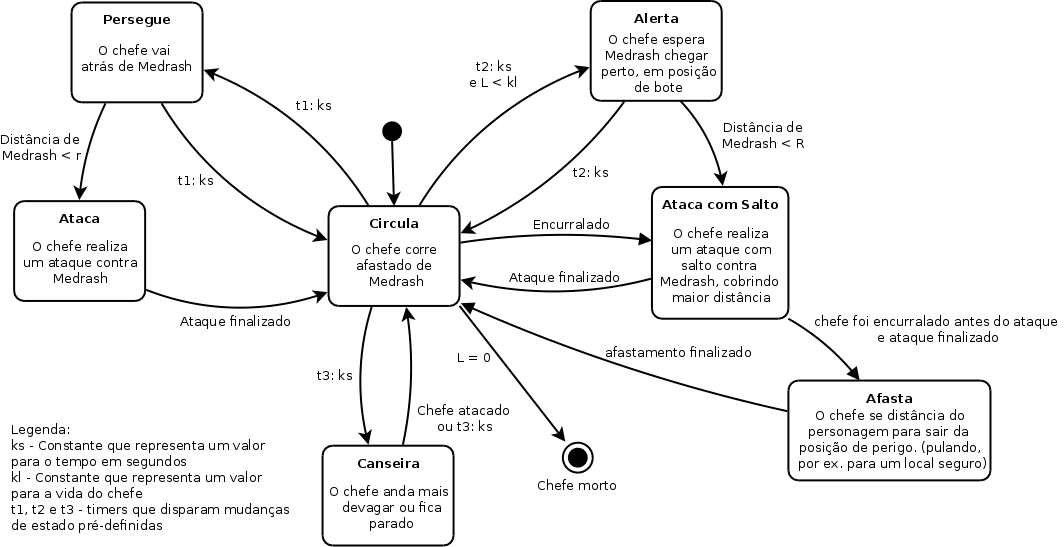
\includegraphics[scale=0.44]{ia_tigre.png}
 \caption{Máquina de estado do Tigre}
 \label{fsm:tigre}
\end{figure}

\subsection{Fase 2}

\subsubsection{Lobo}

O lobo fica patrulhando na montanha. Caso Medrash entre no raio de
deteção do lobo enquanto estiver com a tocha acesa, o lobo fugirá. Caso
Medrash entre no raio de deteção do lobo enquanto estiver com a tocha
apagada, o lobo perseguirá Medrash. Em qualquer um desses casos, se
Medrash ficar muito próximo do lobo, então o lobo atacará Medrash, e
voltará à atividade anterior.
Se, enquanto estiver sendo perseguido, Medrash acender a tocha,
o lobo fugirá. Similarmente, se o lobo estiver fugindo e a tocha se apagar,
o logo passará a perseguir Medrash.

A máquina de estados pode ser vista na figura \ref{fsm:lobo}.

\begin{figure}[!ht]
 \centering
 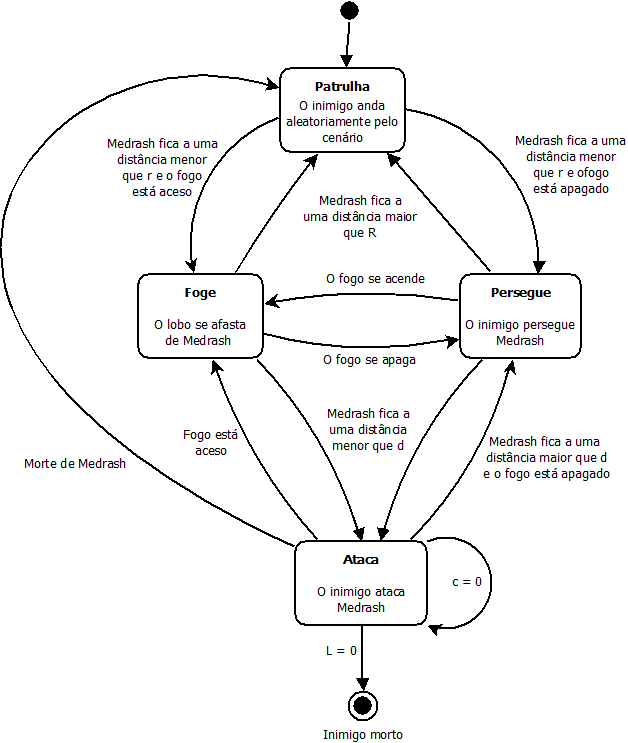
\includegraphics[scale=0.5]{ia_lobo.png}
 \caption{Máquina de estado do Lobo}
 \label{fsm:lobo}
\end{figure}

\subsubsection{Guerreiro}

O guerreiro entra no campo de batalha já perseguindo Medrash. Caso
Medrash esteja próximo do piromaníaco e dentro do raio de ataque do 
guerreiro, então o guerreiro empurrará Medrash.
Se Medrash não estiver muito próximo do piromaníaco, mas estiver dentro
do raio de ataque do guerreiro, então o guerreiro atacará Medrash.

A máquina de estados pode ser vista na figura \ref{fsm:guerreiro}.

\begin{figure}[!ht]
 \centering
 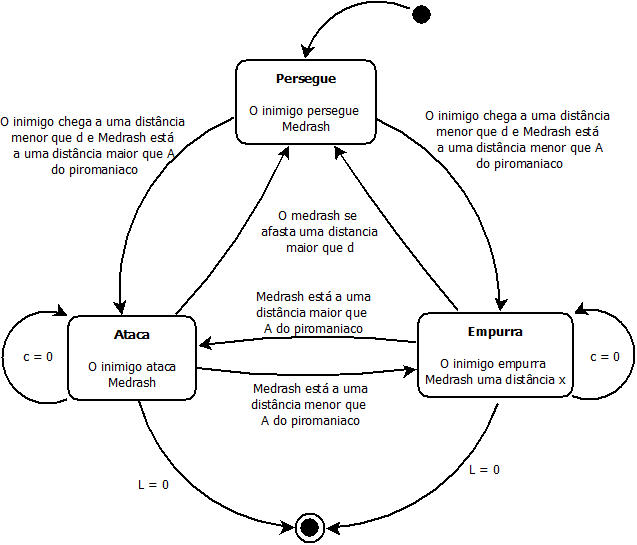
\includegraphics[scale=0.5]{ia_guerreiro.png}
 \caption{Máquina de Estado do Guerreiro}
 \label{fsm:guerreiro}
\end{figure}

\subsubsection{Piromaníaco}

O piromaníaco entra no campo de batalha se deslocando ao local mais
próximo para atear fogo. Seu único objetivo é atear fogo em todos os
locais possíveis. Caso isso aconteça, o jogador perde o jogo.

A máquina de estados pode ser vista na figura \ref{fsm:piromaniaco}.

\begin{figure}[!ht]
 \centering
 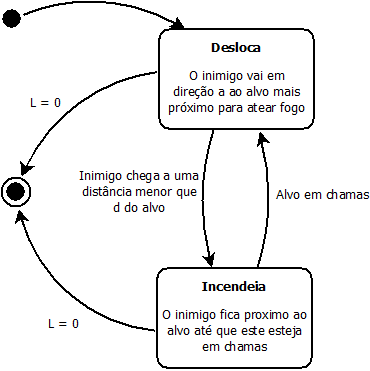
\includegraphics[scale=0.5]{ia_piromaniaco.png}
 \caption{Máquina de Estado do Piromaníaco}
 \label{fsm:piromaniaco}
\end{figure}

\subsection{Fase 3}

\subsubsection{Fanático}

O fanático será instanciado conforme necessário para atacar o Medrash.
Ele já inicia perseguindo Medrash. Quando fica perto o suficiente, ele
ataca Medrash. Se Medrash se afastar, ele volta a perseguí-lo.

A máquina de estados pode ser vista na figura \ref{fsm:fanatico}.

\begin{figure}[!ht]
 \centering
 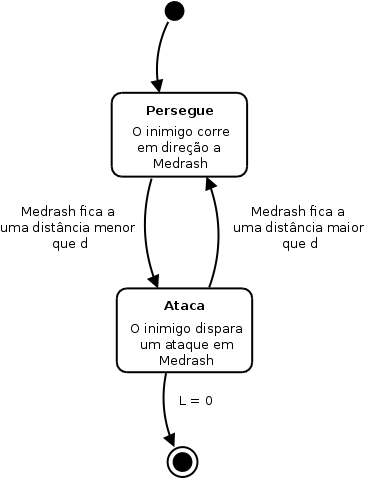
\includegraphics[scale=0.5]{ia_fanatico.png}
 \caption{Máquina de Estado do Fanático}
 \label{fsm:fanatico}
\end{figure}

\subsubsection{Balasar (Chefe)}

O Balasar já inicia na batalha. Inicialmente ele prepara o ataque.
Após alguns segundos, ele investe em direção à Medrash. Seu movimento
é essencialmente retilíneo. Durante o movimento, sua rotação é limitada.
Se Balasar chegar a uma certa distância de Medrash durante a investida,
ele deferirá um ataque contra o mesmo. Medrash pode desviar desse ataque,
mas não pode se defender. Medrash pode fugir da investida, permanecendo
longe da trajetória de Balasar. Nesse caso, Balasar não realizará o ataque.
Depois da investida, bem sucedida ou não, Balasar se afastará.
Ao se afastar o suficiente, Balasar voltará a preparar o ataque.

Após uma certa quantidade de ataques, Balasar irá prender a clava no
chão. Nesse momento, Medrash deve ir atacar as estacas que prendem Sora.
Caso Medrash se aproxime de Balasar, ele será atacado com um chute que
também o afastará. Passado um certo período de tempo, Balasar solta a
clava, e volta a preparar o ataque.

A máquina de estados pode ser vista na figura \ref{fsm:balasar_e1}.

\begin{figure}[!ht]
 \centering
 %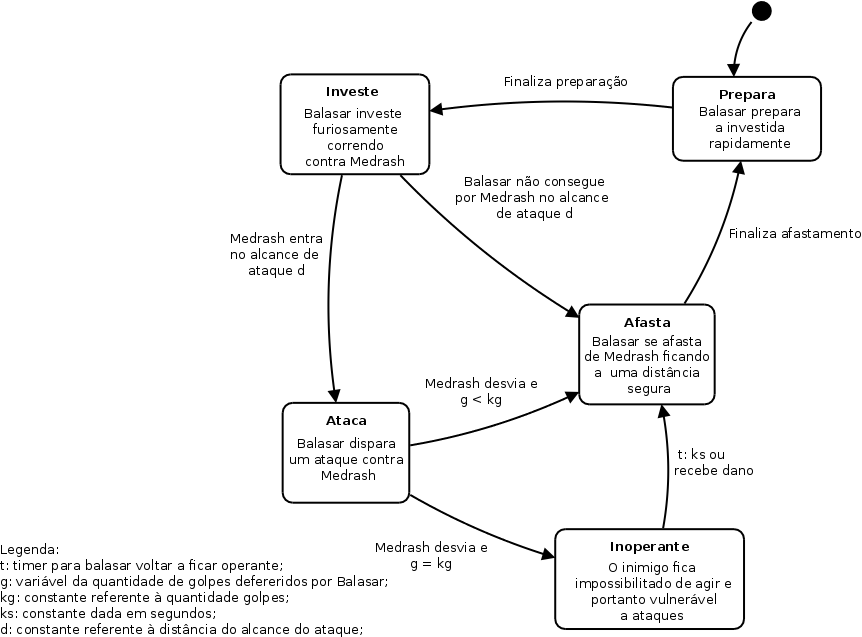
\includegraphics[scale=0.5]{ia_balasar_e1.png}
 \caption{Máquina de Estado do Balasar}
 \label{fsm:balasar_e1}
\end{figure}

O objetivo de Medrash nessa batalha é libertar Sora, destruindo as 
estacas que a prendem. Quando Medrash destruir as estacas suficientemente,
Balasar mudará seu comportamento, se tornando mais agressivo.
Nesse novo comportamento, Balasar dará ataques triplos, investindo contra
Medrash a cada ataque. Os outros aspectos do comportamento são semelhantes
ao comportamento anterior.

A máquina de estados deste novo comportamento pode ser vista na figura
 \ref{fsm:balasar_e2}.

\begin{figure}[!ht]
 \centering
 %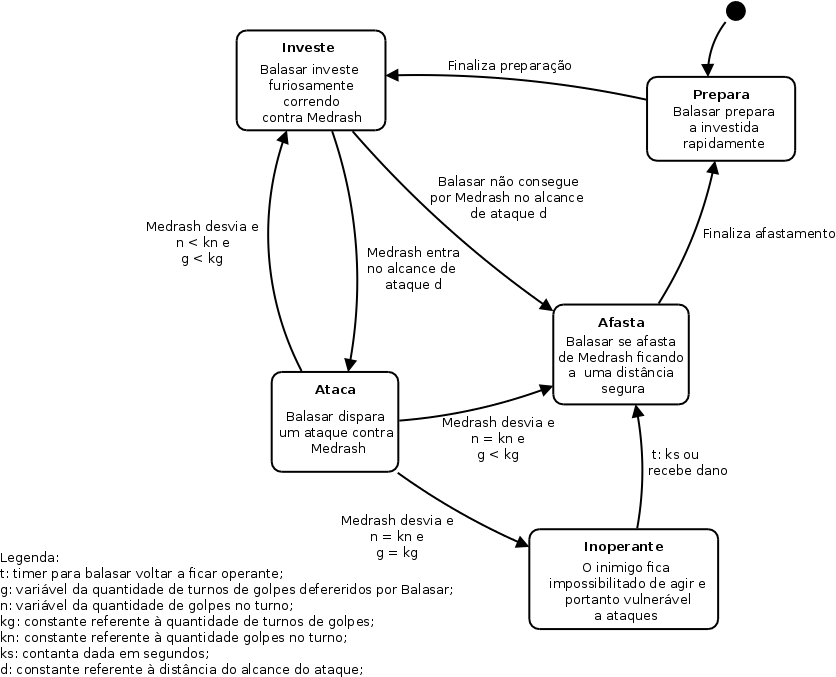
\includegraphics[scale=0.5]{ia_balasar_e2.png}
 \caption{Máquina de Estado do Balasar}
 \label{fsm:balasar_e2}
\end{figure}
% \include{detalhamento}
\section{Testes}
Com o decorrer dos anos, aplicações de software robustas e complexas
 demandam cada vez mais esforços para que se mantenha sua qualidade. A
 engenharia de software é constituída por um grupo de métodos, ferramentas e
 critérios cujo objetivo recai sobre a tentativa de produzir aplicativos
 detentores desta qualidade. Dentre os processos propostos por ela, estão
 aqueles responsáveis por descrever as atividades de teste de software.
   
O teste de software refere-se a um processo de âmbito investigativo, ou
 seja, as ferramentas e métodos propostos  por ele têm por objetivo procurar
 e encontrar problemas presentes em  uma aplicação. Sendo verdade, pode-se
 dizer que trata-se de uma investigação a respeito da qualidade do
 aplicativo dentro do contexto ao qual ele deve operar. Segundo
 \cite{bib:pressman} o objetivo central do teste é o de apontar a existência
 da maior quantidade possível de defeitos que  não foram identificados pelas
 revisões dentro dos limites de prazo e de custo.

Diz-se que um caso de teste é bom quando apresenta grande probabilidade de
 revelar a presença de um defeito ainda não descoberto. Portanto, pode-se
 dizer que um teste é bem-sucedido quando aponta e verifica a presença de um
 defeito de maneira satisfatória.
 
Um ponto de vista errôneo geralmente extraído de um aplicativo
 disponibilizado para ser comercializado é de que ele deve funcionar
 corretamente, sem a presença de erros. A complexidade envolvida em sua
 codificação, somada aos profissionais presentes, torna impraticável a
 possibilidade de provar esta corretitude.
 
As falhas de aplicativos podem ser geradas por uma grande gama de motivos,
 dentre os quais, especificações de requisitos erradas, implementações
 incorretas e plataformas de hardware não suportáveis. 

No âmbito do teste de software há uma distinção clara entre os conceitos de
 defeito, erro e falha, cada qual com suas características e
 particularidades. Uma falha é uma condição anormal na saída que era
 esperada por um componente do software, ou seja, algo que é visível ao
 usuário. O defeito é algo causador da falha e, portanto, pode-se dizer que
 se caracteriza por ser algum problema com o código do software. Por fim, o
 erro é um estado inconsistente que se propaga pelo sistema após o exercício
 de um defeito. Sendo verdade, diz-se que o erro pode ou não acarretar em
 uma falha devido a fatores tais como redundância de processamento.

Pressman discorre sobre a atividade de teste da seguinte maneira: “Se
 realmente fossemos bons para programar não haveria bugs. Se existem bugs, é
 porque somos ruins naquilo que fazemos e, se somos ruins nisso devemos
 sentir-nos culpados por isso. Assim, a atividade de teste e o projeto de
 casos de teste são 
uma admissão de falha, o que promove uma boa dose de culpa. O tédio de
 testar é apenas uma punição por nossos erros”. 

As principais considerações do teste de software são: 

\begin{itemize}
\item Para ser eficaz o teste deve ser cuidadosamente desenhado;
\item Testes improvisados devem ser evitados;
\item Resultados devem ser inspecionados e comparados com resultados esperados;
\item Desenvolvedores não são as pessoas mais indicadas para testar seu próprio produto;
\item Testadores independentes são importantes;
\end{itemize}

No que diz respeito às abordagens para o teste de software pode-se dizer que
 há três: teste de caixa branca, de caixa preta e caixa cinza.

O teste caixa preta, do inglês \textit{Black Box}, ou teste funcional,
 caracteriza-se por não considerar o código fonte da aplicação ao efetuar os
 testes. Responsabiliza-se por determinar se os requisitos foram total ou
 parcialmente satisfeitos com a verificação dos resultados obtidos, deixando
 de lado o modo como ocorreu o processamento. Também demonstra quais são as
 funções do software que encontram-se operacionais, ou seja, aquelas que
 produzem a saída esperada. Dentre as principais técnicas que utilizam-se
 desta abordagem cita-se o particionamento de equivalência e a análise do
 valor limite.

O teste caixa branca, do inglês \textit{White Box}, ou teste estrutural, de
 maneira oposta ao que ocorre com o caixa preta, considera o código da
 aplicação na aplicação das atividades de teste. Responsabiliza-se por
 determinar defeitos na estrutura interna do programa por meio do exercício
 dos caminhos de execução, com a execução de conjuntos específicos de
 condições ou laços. Dentre as principais técnicas
 que utilizam-se desta abordagem cita-se o teste de caminho básico, o qual
 utiliza um grafo de programa para denotar as instruções presentes no código
 fonte.

O teste caixa cinza, do inglês \textit{Gray Box}, caracteriza-se por ser um
 híbrido entre os dois anteriormente descritos, caixa branca e preta, por
 apresentar elementos e características presentes em ambos.

Para o jogo ``As Crônicas de Medrash'' a ser desenvolvido, testes funcionais
 serão realizados em detrimento dos estruturais. O jogo será testado de
 acordo com as especificações presentes no documento de \textit{Game
 Design}. Serão criado casos de testes para exercitar aspectos variados
 referentes ao jogo tais como fluxo das fases, inteligência artificial do
 inimigos e comportamentos do personagem principal.
 
A criação e execução dos casos de testes deverá ser feita por pessoal
 especializado. A correção dos eventuais problemas encontrados será cargo do
 desenvolvedor responsável. Poderá também haver o re-teste no âmbito de se
 verificar se o problema foi realmente corrigido ou se não gerou novos com
 a solução aplicada.

\bibliographystyle{plain}
\bibliography{gdd}

\end{document}

